%\PassOptionsToPackage{draft}{graphicx}
\documentclass[14pt]{beamer}

\usetheme{metropolis}
\usepackage{appendixnumberbeamer}

\usepackage{booktabs}
\usepackage[scale=2]{ccicons}

\usepackage{pgfplots}
\usepgfplotslibrary{dateplot}

\usepackage{xspace}
\newcommand{\themename}{\textbf{\textsc{metropolis}}\xspace}

\usepackage{hyperref}

\graphicspath{{./images/}}

\title{Learning To Drive}
\subtitle{Pedestrian Detection for Self Driving Cars}
\date{\tiny\today}
\author{Simone Rossi \& Matteo Romiti}
\institute{EURECOM, Ecole d'Ing\'enieur et Centre de Recherche en Telecommunications}
 \titlegraphic{\hfill
\includegraphics[height=1.5cm]{logo.png}}

\begin{document}

\maketitle

\begin{frame}{Table of contents}
  \small
  \setbeamertemplate{section in toc}[sections numbered]
  \tableofcontents[]%hideallsubsections
\end{frame}

%\section{Introduction}

\begin{frame}[fragile]{Metropolis}

  The \themename theme is a Beamer theme with minimal visual noise
  inspired by the \href{https://github.com/hsrmbeamertheme/hsrmbeamertheme}{\textsc{hsrm} Beamer
  Theme} by Benjamin Weiss.

  Enable the theme by loading

  \begin{verbatim}    \documentclass{beamer}
    \usetheme{metropolis}\end{verbatim}

  Note, that you have to have Mozilla's \emph{Fira Sans} font and XeTeX
  installed to enjoy this wonderful typography.
\end{frame}


\begin{frame}[fragile]{Sections}
  Sections group slides of the same topic

  \begin{verbatim}    \section{Elements}\end{verbatim}

  for which \themename provides a nice progress indicator \ldots
\end{frame}


\section{Histograms of Oriented Gradients}

\begin{frame}{Histograms of Oriented Gradients}
  \metroset{block=fill}
\center
\only<1>{
  \begin{alertblock}{\textbf{Why?}}
  One of the most well known methods for feature extraction for human detection in
  computer vision, it is very versatile and it can be applied in different contexts.
  Ofter it is used as metrix to compare more sophisticated methods.
  \end{alertblock}
}

\only<2>{
  \begin{exampleblock}{\textbf{Idea?}}
  Describe the local behaviour of the gradient applied to an image, in ordet to
  emphasize well defined geometric structures and edges. A local object appearance
  and shape can be characterized by the distribution of local intensity gradients or
  edge directions, even without knowledge of the corresponding gradient.
\end{exampleblock}

}

\only<3>{

\begin{exampleblock}{\textbf{How?}}
  Divide the image window into small spatial regions (\textit{cells}), accumulate
  a 1D \textit{histogram} of gradient directions over the pixels of the cell and
  normalize the result over a \textit{block} of cells for better invariance to illumination.
\end{exampleblock}
}

\end{frame}


\begin{frame}{Algorithm for HOG Extraction}
%\documentclass{standalone}
%\usepackage{tikz}
%%include other needed packages here
%\begin{document}

\small
\tikzstyle{block} = [rectangle, draw, %fill=blue!20,
                  text width=3.1em, text centered, rounded corners, minimum height=2.5em]

\tikzstyle{block_invisible} = [rectangle,text width=7em, text centered, rounded corners]
\tikzstyle{line} = [draw, -latex]

\center

\begin{tikzpicture}[node distance = 2.25cm,scale=0.6]

    % Place nodes
    \node [block_invisible] (input_image) {\scriptsize \textbf{Input image} \\ (to be analyzed)};
    \node [block, above of=input_image, node distance=1.5cm] (normalizzazione_gamma_colore) {{\scriptsize Preproc.}};
    \node [block, right of=normalizzazione_gamma_colore] (gradiente) {\scriptsize Gradient};
    \node [block, text width=3.5em, right of=gradiente] (pesatura_bins) {\scriptsize Histograms};
    \node [block, text width=4em, right of=pesatura_bins] (normalizzazione_blocco) {\scriptsize Normalization};
    \node [block_invisible, below of=normalizzazione_blocco,node distance=1.5cm] (classificatore) {\scriptsize \textbf{Feature vectors} \\ (to the classifier)};

    % Draw edges
    \path [line] (input_image) -- (normalizzazione_gamma_colore);
    \path [line] (normalizzazione_gamma_colore) -- (gradiente);
    \path [line] (gradiente) -- (pesatura_bins);
    \path [line] (pesatura_bins) -- (normalizzazione_blocco);
    \path [line] (normalizzazione_blocco) -- (classificatore);


\end{tikzpicture}

\end{frame}

\begin{frame}{Noise Reduction}
\only<1>{
  Due to the intrinsic randomness nature of an acquisition system, generally an image
  is always affected by an high frequency noise (likely modeled as AWGN).\\
  \vspace{0.25cm}
  It may be useful to reduce the noise level before starting to extract features.
}

\only<2>{
  General noise reduction filter: \textbf{Gaussian Filter}
  \begin{equation}
    g(x,y) = \dfrac{1}{2\pi\sigma^2}\exp{\left(-\dfrac{x^2+y^2}{2\sigma^2}\right)}
  \end{equation}
  \begin{figure}
    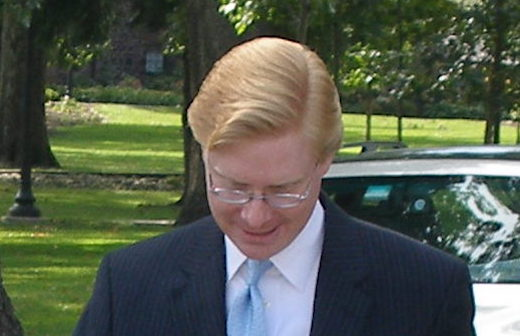
\includegraphics[width=.4\textwidth]{no_filter.jpg}
    \hspace{1mm}
    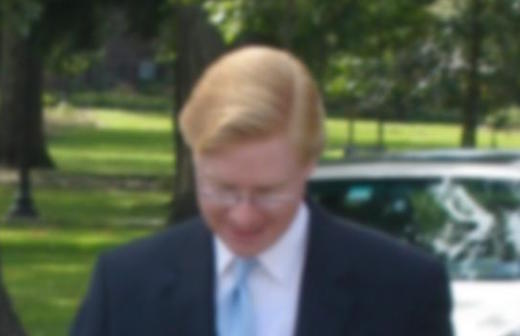
\includegraphics[width=.4\textwidth]{filter.jpg}
  \end{figure}
}
\end{frame}


\begin{frame}{Gradient Computation}
\tikzstyle{block_a} = [rectangle, draw, %fill=blue!20,
     text width=2em, text centered, rounded corners, minimum height=3em]
\tikzstyle{block_b} = [rectangle, draw, %fill=blue!20,
     text width=7em, text centered, rounded corners, minimum height=5em]
\tikzstyle{line} = [draw, -latex]


\footnotesize

\begin{tikzpicture}[node distance = 2.5cm, every text node part/.style={align=center}]
    % Place nodes
    \node [] (input_image) at (0,0) {$I(j,k)$};
    \node [] (node1) at (1.5,0) {};

    \node [block_a, above right of=node1,  node distance=2cm] (gradiente_x) {$h_x$};
    \node [] () at (5,1.65){$G_x(j,k)=I(j,k)*h_x$};

    \node [block_a, below right of=node1, node distance=2cm] (gradiente_y) {$h_y$};
    \node [] () at (4.75,-1.7){$G_y(j,k)=I(j,k)*h_y$};
    %\node [] (node2) at (4,0) {};
    \node [block_b] (combinazione) at (6,0) {$G=\sqrt{G_x^2+G_y^2}$ \\ $\theta=atan\left(\tfrac{G_y}{G_x}\right)$};
    \node[right of = combinazione](uscita){$\mathbf{G}(j,k)$};

    % Draw edges
    \path [draw, -] (input_image) -- (node1);
    \path [line] (node1) |- (gradiente_x);
    \path [line] (node1) |- (gradiente_y);
    \path [line] (gradiente_x) -| (combinazione);
    \path [line] (gradiente_y) -| (combinazione);
     %\path [line] (node2) -- (combinazione);
     \path [line] (combinazione) -- (uscita);
\end{tikzpicture}

\end{frame}


\begin{frame}{Histograms}

\only<1>{
  \begin{figure}[!ht]
  \centering
  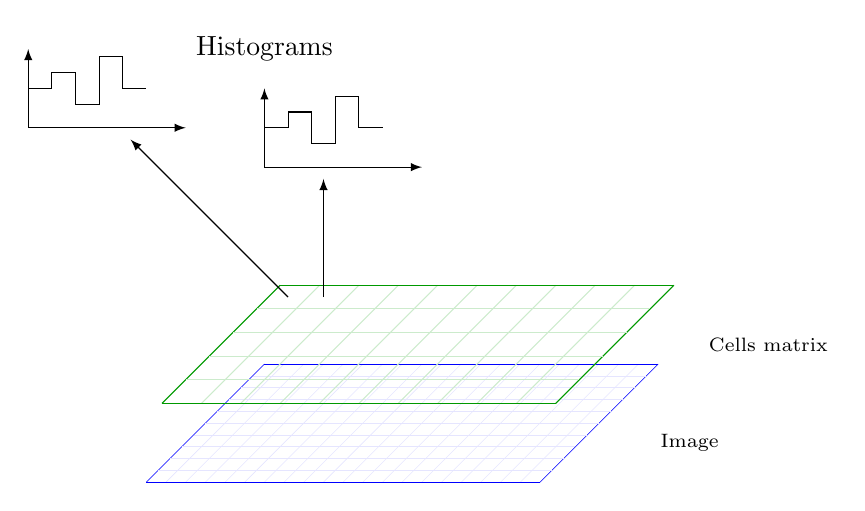
\begin{tikzpicture}[scale=1]

\foreach \x in {0,0.25,0.5,...,5} \draw[color=blue!10,very thin] (\x,0)--+(-1.5,-1.5);
\foreach \x in {0,5} \draw[color=blue,very thin] (\x,0)--+(-1.5,-1.5);

\foreach \y in {0,0.15,0.3,...,1.6 } \draw[color=blue!10,very thin] (-1*\y,-\y)--+(5,0);
\foreach \y in {0,1.5 } \draw[color=blue,very thin] (-1*\y,-\y)--+(5,0);

\node[] at (5.4,-1){{\scriptsize Image}};

\foreach \x in {0,0.5,1,...,5} \draw[color=green!60!black!20,thin] (\x+0.2,0+1)--+(-1.5,-1.5);
\foreach \x in {0,5} \draw[color=green!60!black,thin] (\x+0.2,0+1)--+(-1.5,-1.5);

\foreach \y in {0,0.3,0.6,...,1.6 } \draw[color=green!60!black!20,thin] (-1*\y+0.2,-\y+1)--+(5,0);
\foreach \y in {0,1.5 } \draw[color=green!60!black,thin] (-1*\y+0.2,-\y+1)--+(5,0);
\node[] at (6.4,0.25){{\scriptsize Cells matrix}};


\draw[-latex](0.3,0.85)--+(-2,2);
\draw[-latex](-3,3)--+(2,0);
\draw[-latex](-3,3)--+(0,1);
\draw[](-3,3.5)--+(0.3,0)--+(0.3,0.2)--+(0.6,0.2)--+(0.6,-.2)--+(0.9,-.2)--+(0.9,.4)--+(1.2,.4)--+(1.2,0)--+(1.5,0);

%
%
\draw[-latex](0.75,0.85)--+(0,1.5);
\draw[-latex](0.,2.5)--+(2,0);
  \draw[-latex](0.,2.5)--+(0,1);
  \draw[](0,3)--+(0.3,0)--+(0.3,0.2)--+(0.6,0.2)--+(0.6,-.2)--+(0.9,-.2)--+(0.9,.4)--+(1.2,.4)--+(1.2,0)--+(1.5,0);
  \node[] at (0,4){Histograms};
\end{tikzpicture}

  \caption{Spatial distribution of histograms and cells}
  \end{figure}
}

%------------------ SLIDE 2 ------------------
\only<2>{
  All the histograms are built as follows ($k=1,\ldots,n_\theta$):
  \begin{equation}
  H_c(k)=\sum_i\sum_jf[G(i,j)]\delta(\phi_{k-1}<\theta(i,j)<\phi_k)
  \end{equation}

  \begin{itemize}
  \item $n_\theta$ \emph{angle bins} uniformely (?) distributed
  \item The vote is a function of the gradient magnitude at the pixel $f(G)$, either the
        magnitude itself, its square, its square root, ...
  \end{itemize}
}
\end{frame}

\begin{frame}{Normalization}

\only<1>{
  \begin{figure}[!ht]
  \centering
  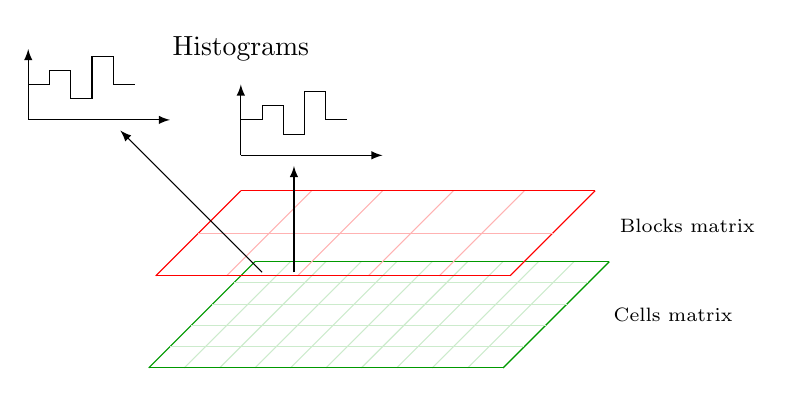
\begin{tikzpicture}[scale=0.9]
  
	\foreach \x in {0,0.5,1,...,5} \draw[color=green!60!black!20,thin] (\x+0.2,0+1)--+(-1.5,-1.5);
  \foreach \x in {0,5} \draw[color=green!60!black,thin] (\x+0.2,0+1)--+(-1.5,-1.5);

  \foreach \y in {0,0.3,0.6,...,1.6 } \draw[color=green!60!black!20,thin] (-1*\y+0.2,-\y+1)--+(5,0);
  \foreach \y in {0,1.5 } \draw[color=green!60!black,thin] (-1*\y+0.2,-\y+1)--+(5,0);
  \node[] at (6.1,0.25){{\scriptsize Cells matrix}};

	\foreach \x in {0,1,2,...,5} \draw[color=red!30,thin] (\x,0+2)--+(-1.2,-1.2);
  \foreach \x in {0,5} \draw[color=red,thin] (\x,0+2)--+(-1.2,-1.2);

  \foreach \y in {0,0.6,1.2 } \draw[color=red!30,thin] (-1*\y,-\y+2)--+(5,0);
  \foreach \y in {0,1.2 } \draw[color=red,thin] (-1*\y,-\y+2)--+(5,0);
  \node[] at (6.3,1.5){{\scriptsize Blocks matrix}};

	\draw[-latex](0.3,0.85)--+(-2,2);
	\draw[-latex](-3,3)--+(2,0);
	\draw[-latex](-3,3)--+(0,1);
	\draw[](-3,3.5)--+(0.3,0)--+(0.3,0.2)--+(0.6,0.2)--+(0.6,-.2)--+(0.9,-.2)--+(0.9,.4)--+(1.2,.4)--+(1.2,0)--+(1.5,0);

	\draw[-latex](0.75,0.85)--+(0,1.5);
	\draw[-latex](0.,2.5)--+(2,0);
  \draw[-latex](0.,2.5)--+(0,1);
  \draw[](0,3)--+(0.3,0)--+(0.3,0.2)--+(0.6,0.2)--+(0.6,-.2)--+(0.9,-.2)--+(0.9,.4)--+(1.2,.4)--+(1.2,0)--+(1.5,0);
  \node[] at (0,4){Histograms};

\end{tikzpicture}

  \caption{Spatial distribution of histograms, cells and blocks}
  \end{figure}
}

\only<2>{
  \small
  \metroset{block=fill}
  \begin{alertblock}{\textbf{Why?}}
  Gradient strengths vary over a wide range owing to local variations
  in illumination and foreground-background contrast, so effective local contrast
  normalization turns out to be essential for good performance.
  \end{alertblock}

  %\vspace{0.5cm}

  Possible normalization scheme:
  \begin{equation}
  H(c,k)= \frac{H_{1}(c,k)}{\left ( \sum_{c_i\in N_c} \sqrt{\|H_{1}(c_i)\|^2_2+\varepsilon^2}\right )}
  \end{equation}
  where $N_c$ is the set of all cells in a block.
}
\end{frame}

\begin{frame}{Results}

  \only<1>{
    \center
    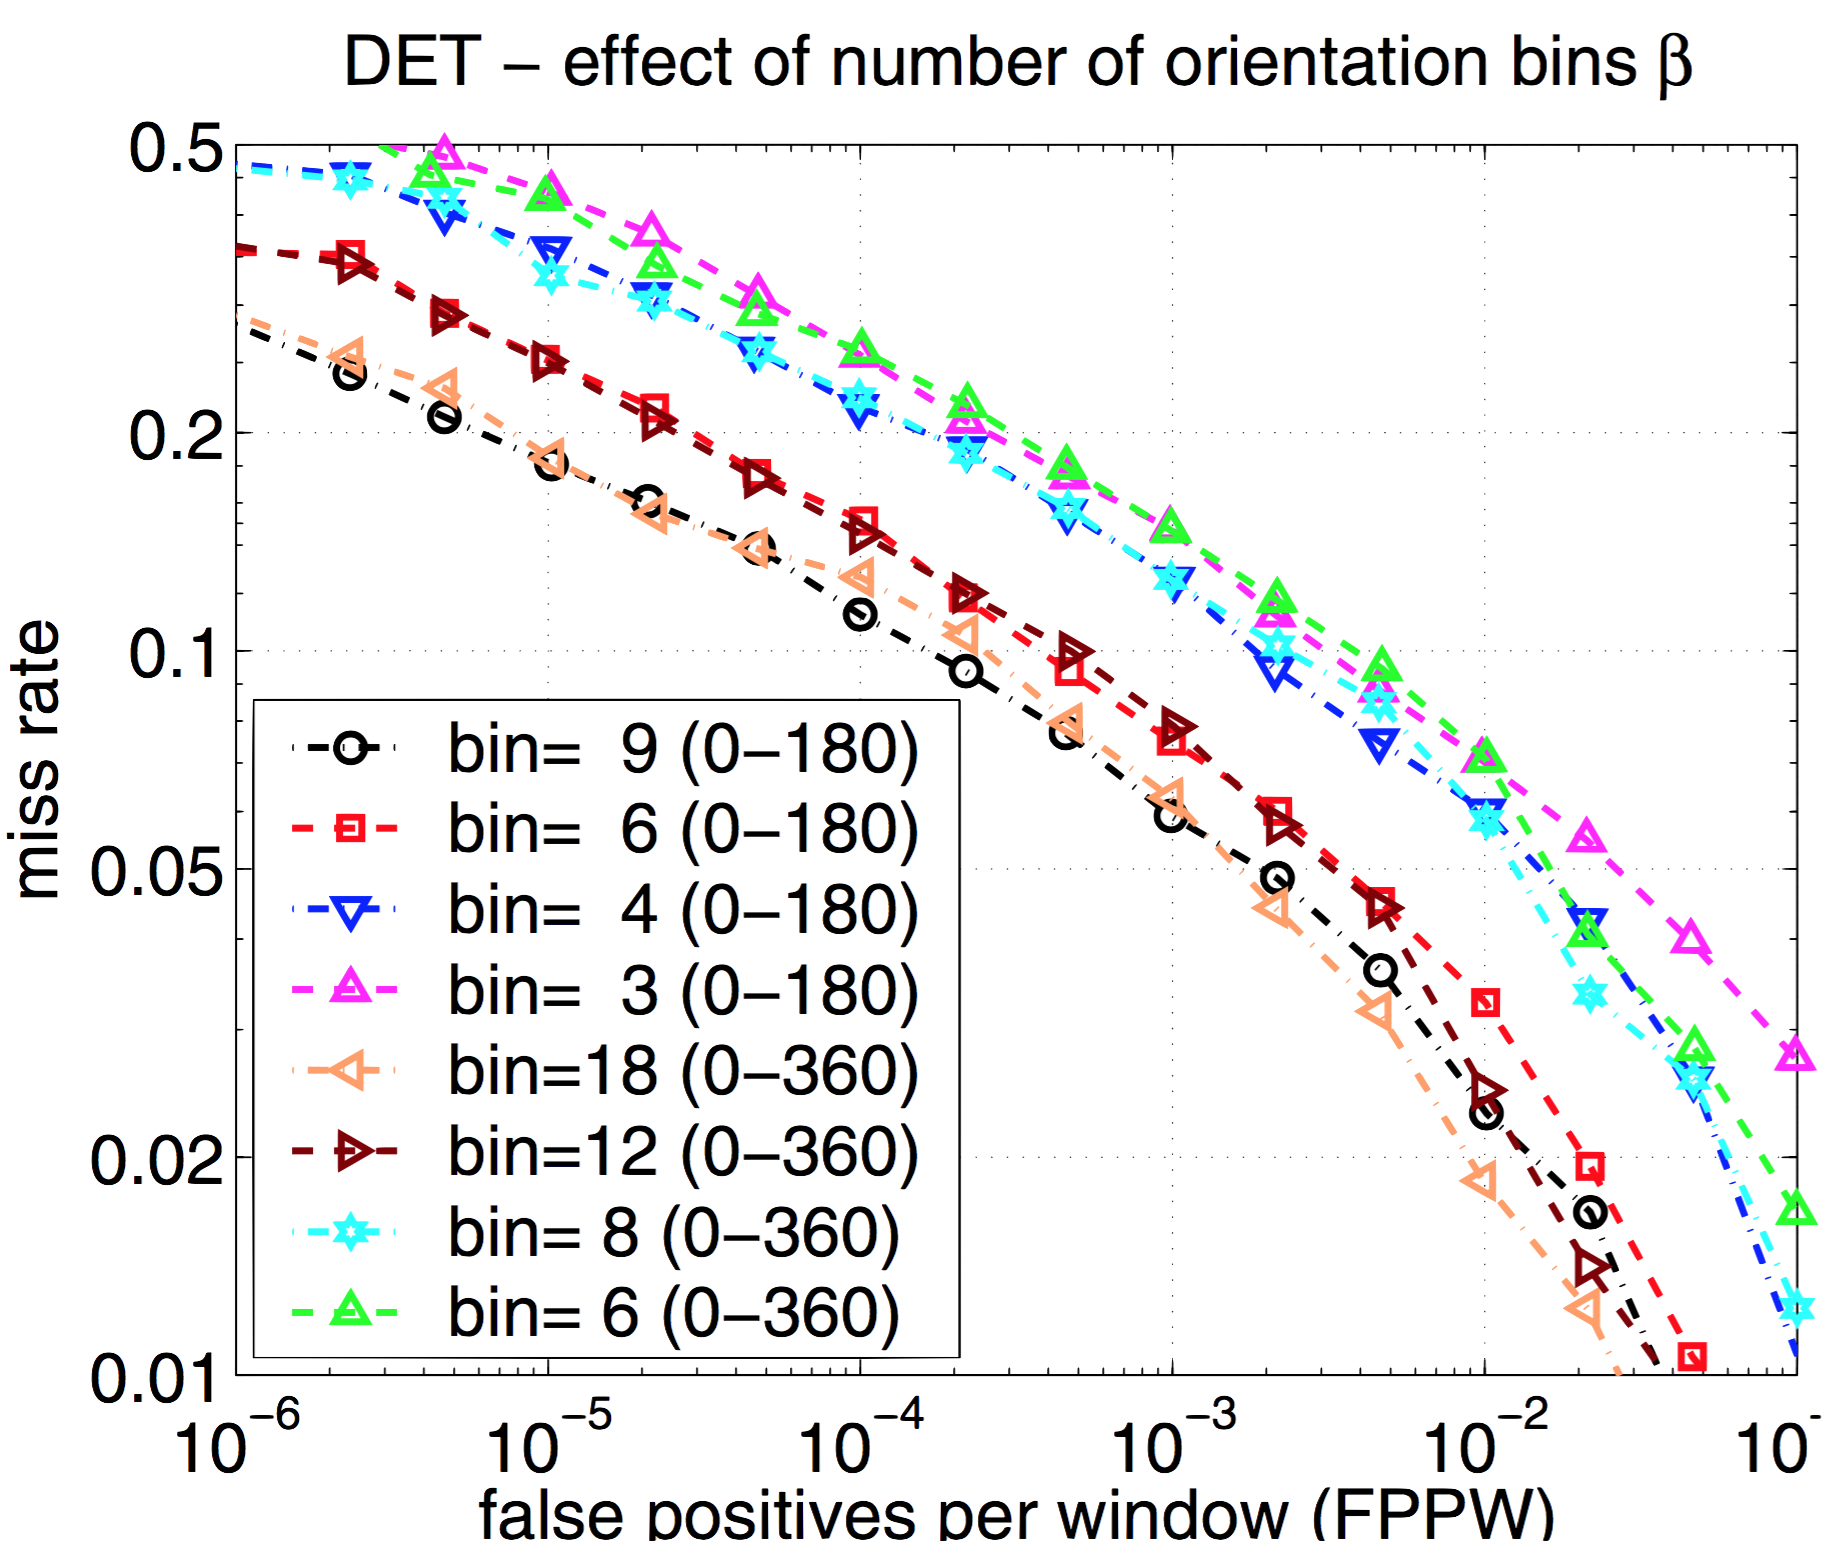
\includegraphics[width=0.75\textwidth]{HOG_result1.png}
  }

  \only<2>{
    \center
    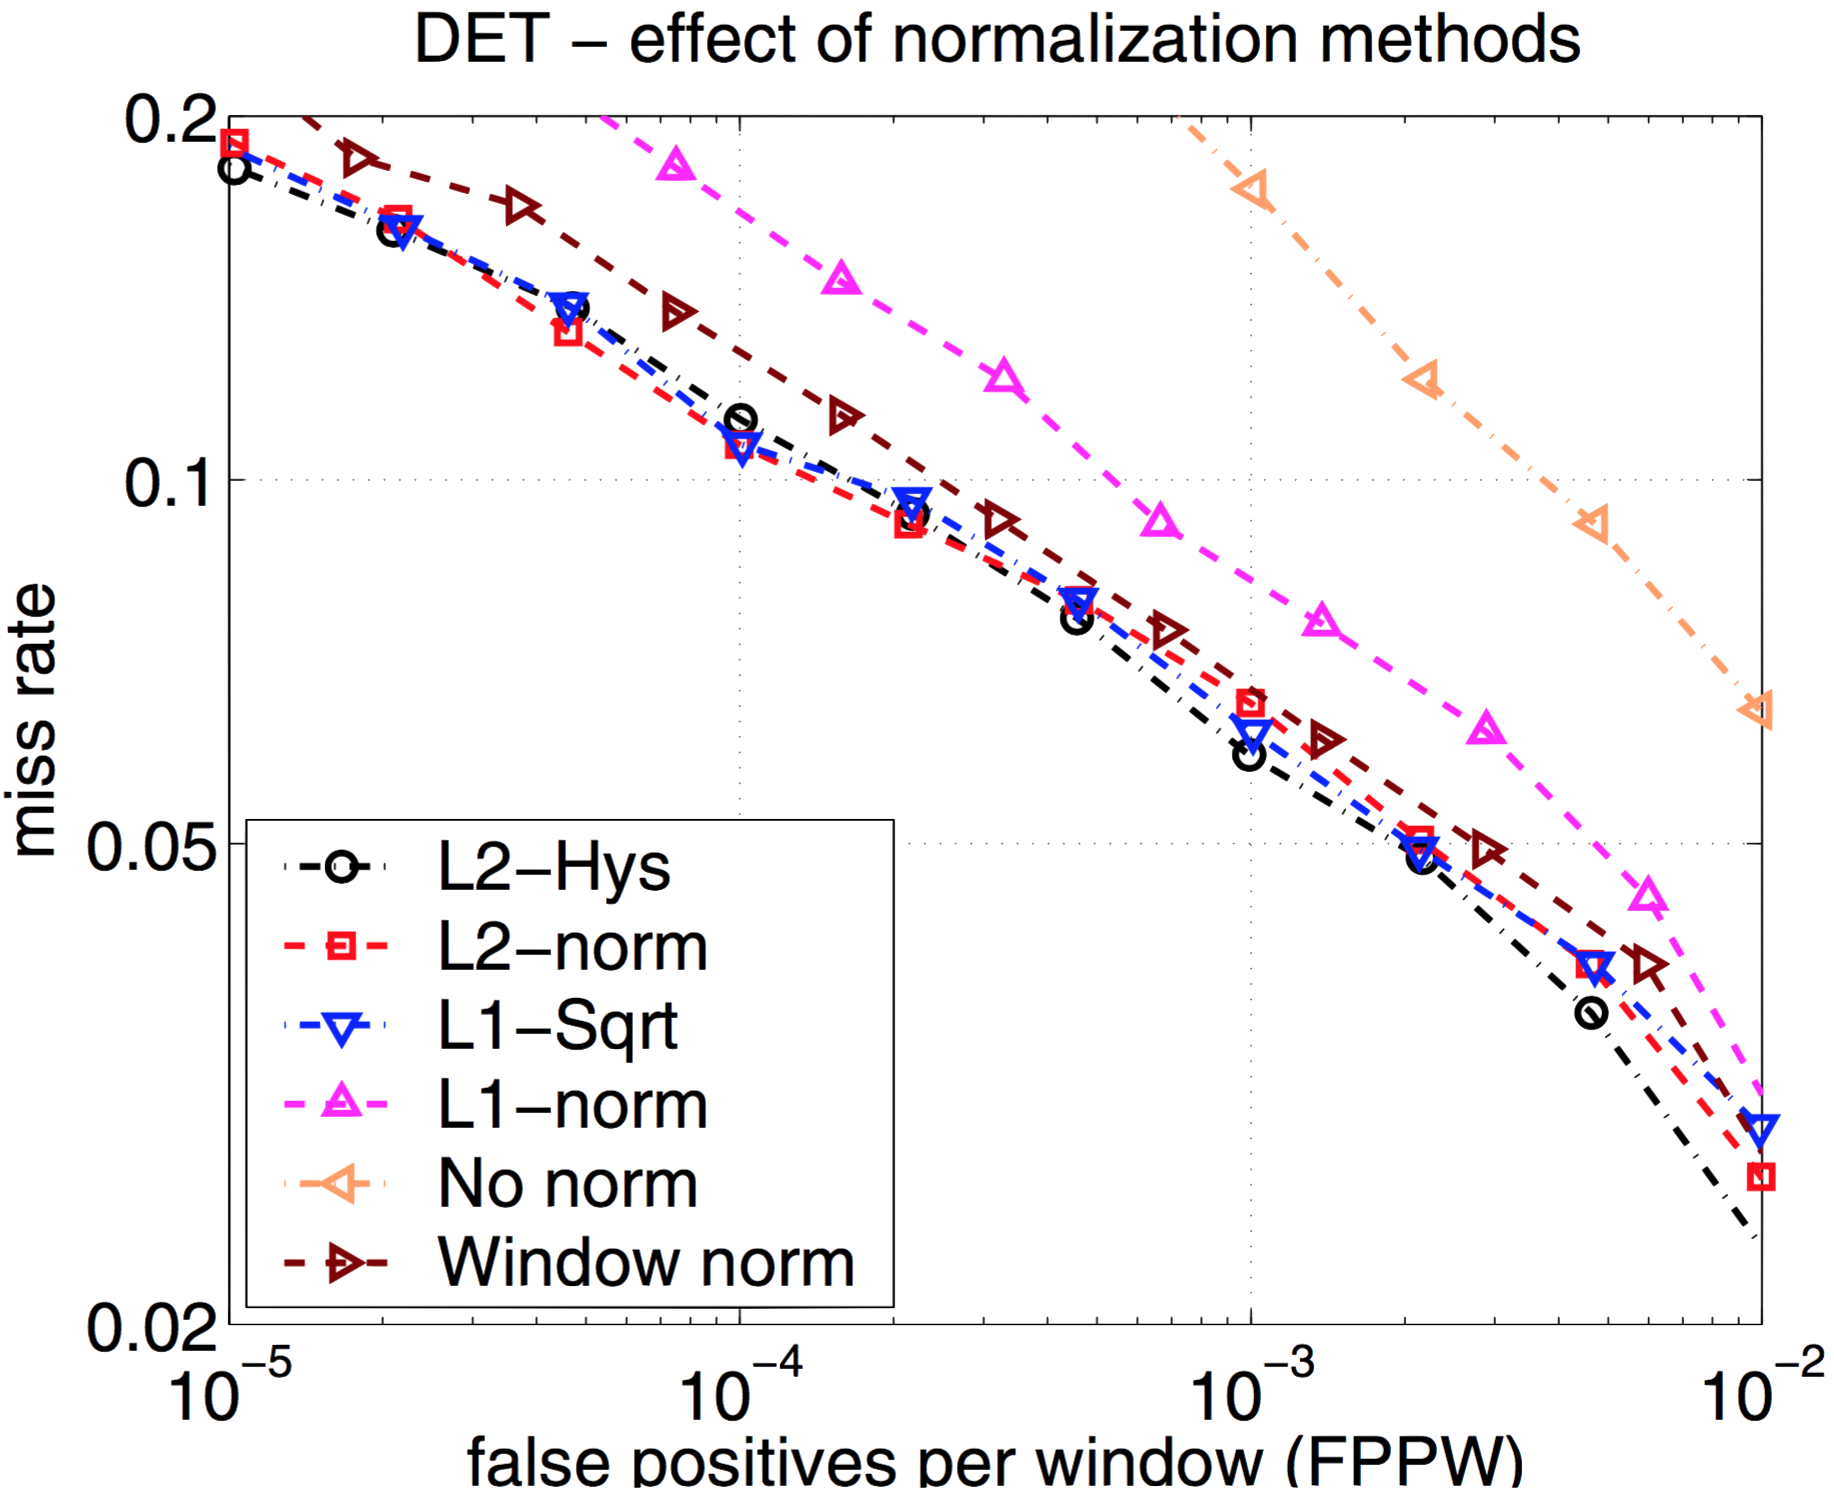
\includegraphics[width=0.75\textwidth]{HOG_result2.png}
  }

  \only<3>{
    \center
    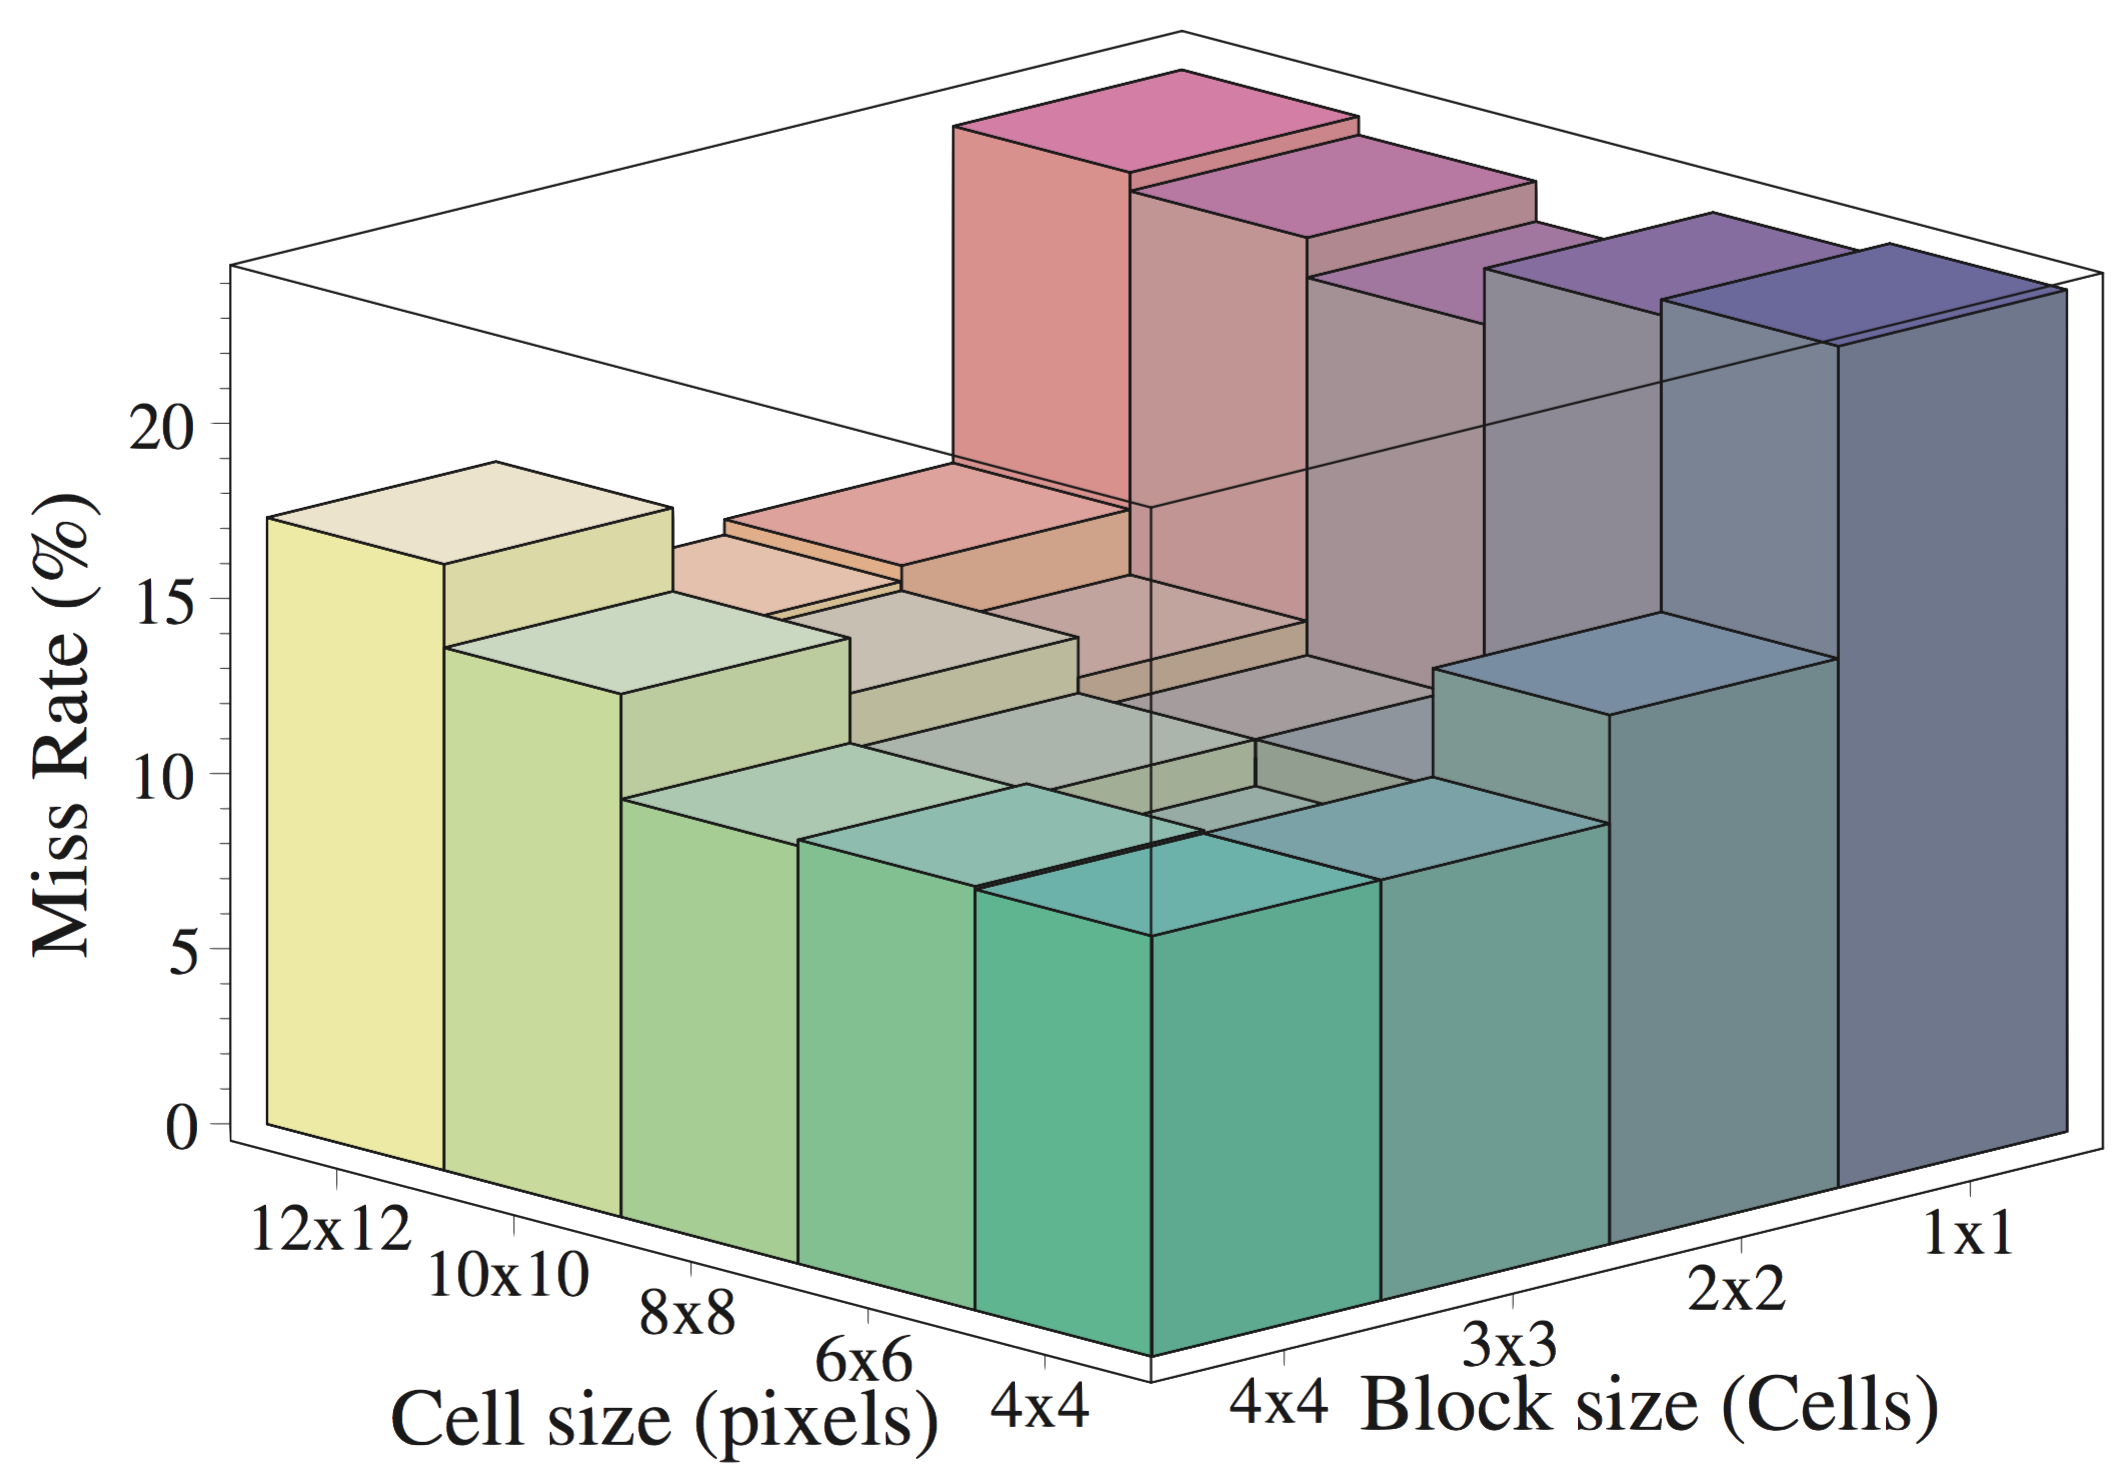
\includegraphics[width=0.75\textwidth]{HOG_result3.png}\\
    \small
    The miss rate at $10^{-4}$ FPPW as the cell and block sizes change.\\
    %3 x 3 blocks of 6 x 6 pixel cells perform best,
    %with 10.4\% miss rate.
  }

\end{frame}

\begin{frame}[standout]
  \huge Demo
\end{frame}

\begin{frame}{Demo}
  \centering
  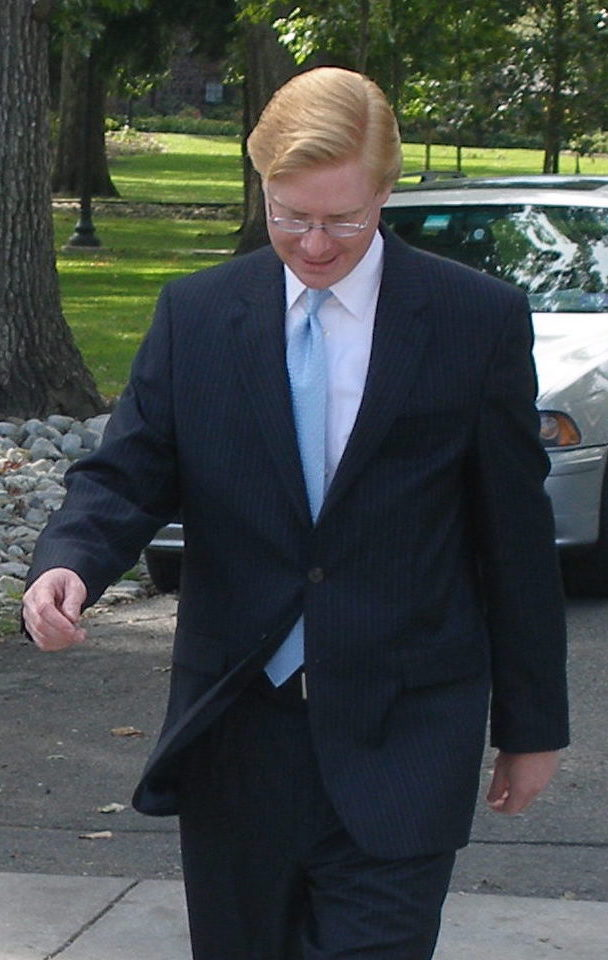
\includegraphics[height = .70\textwidth]{pedestrian.jpg}
  \hspace{2mm}
  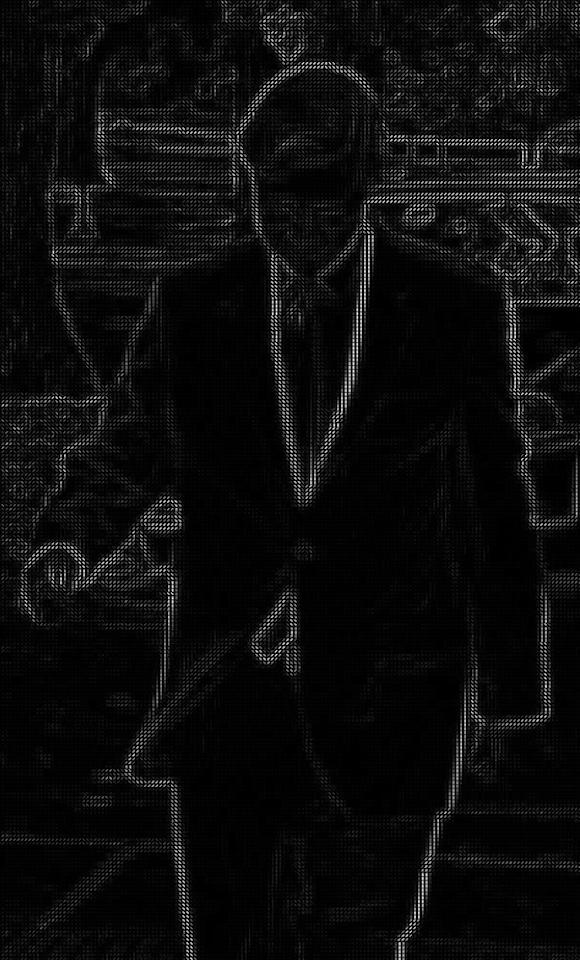
\includegraphics[height = .70\textwidth]{pedestrian_hog.jpeg}
\end{frame}

\begin{frame}{Summary}
  \small
  The HOG representation has several advantages. It captures gradient
  structure that is characteristic of local shape, with a representation invariant
  to local geometric and photometric transformations: translations or rotations make little difference
  if they are much smaller that the local spatial or orientation bin size. \\
  \vspace{5mm}
  For \textit{human detection}, \textbf{fine orientation sampling} and \textbf{strong
  local photometric normalization} turns out to be the best strategy: it permits body
  segments to change appearance and move from side to side quite a lot provided
  that they maintain an upright orientation.

\end{frame}


\begin{frame}[plain]
  \begin{tikzpicture}[remember picture,overlay]
    \node[at=(current page.center)] {
      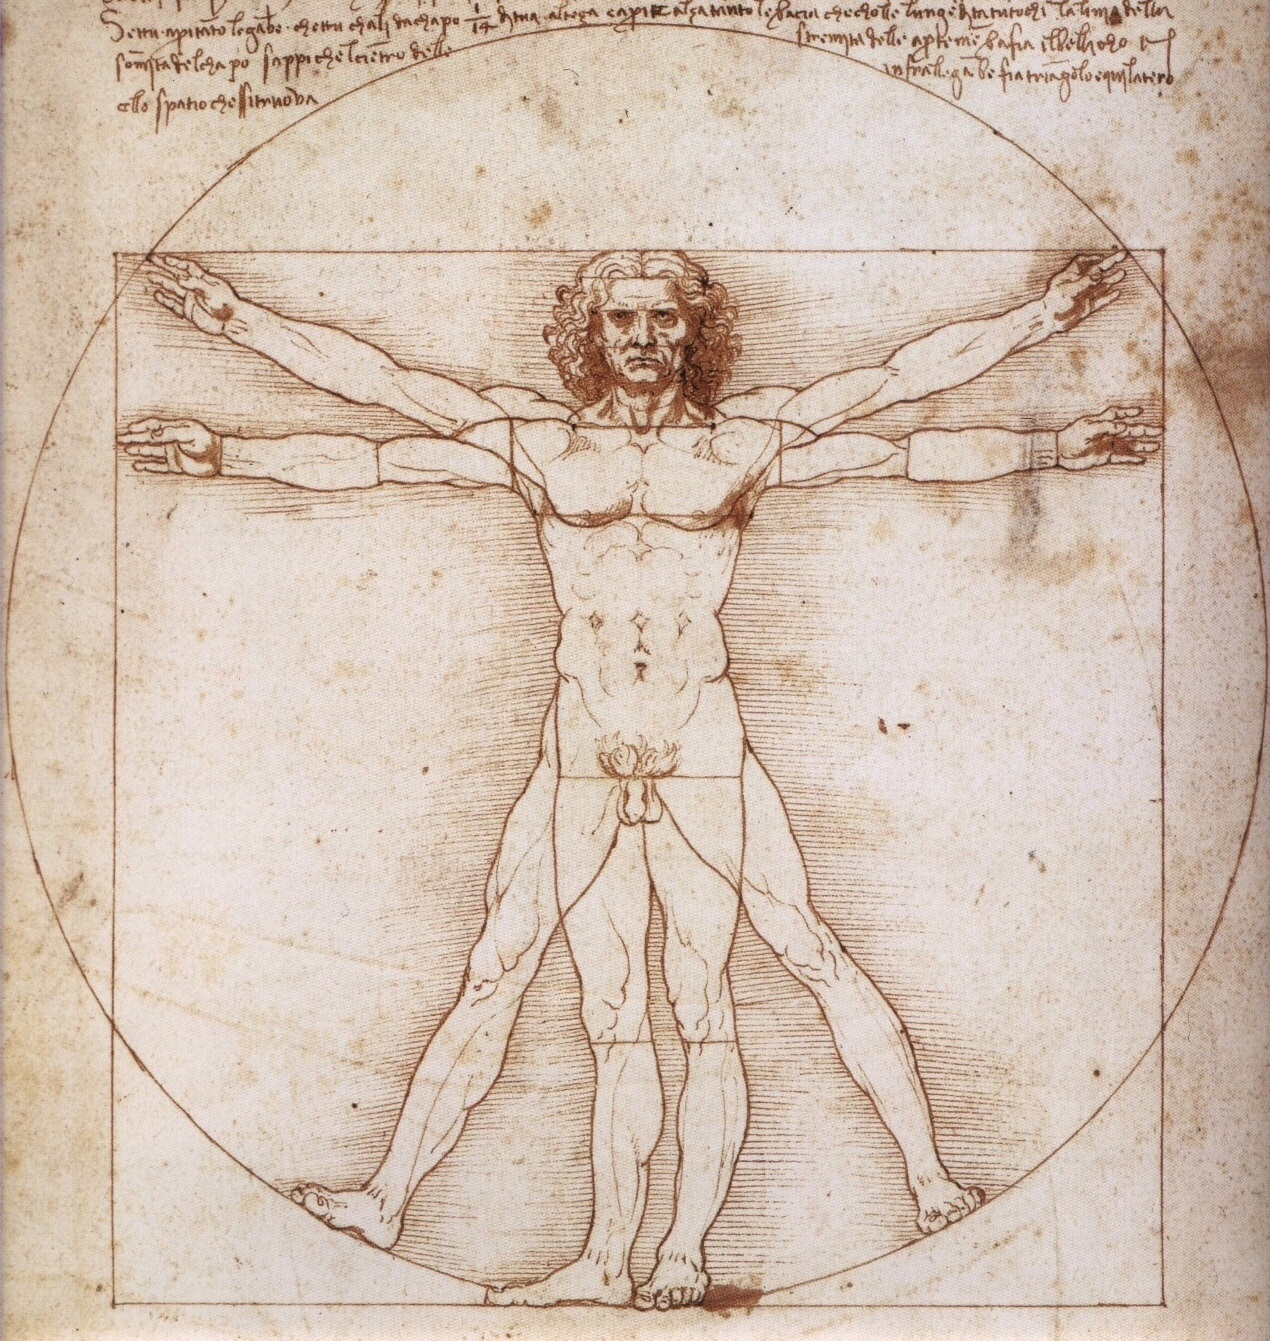
\includegraphics[width=\paperwidth]{uomo_vitruviano.jpg}
    };
  \end{tikzpicture}
\end{frame}

\section{Part-Based Model for Object Detection}

\begin{frame}{Part-Based Model}
  \metroset{block=fill}
  \begin{block}{Idea}
    An object is made of a set of specific sub-blocks.
  \end{block}
  \pause
  \begin{block}{Pictorial structure}
    Pictorial structures represent objects by a collection of parts arranged in
    a deformable configuration.
  \end{block}
\end{frame}


\begin{frame}{Pictorial Structures}
  \centering
  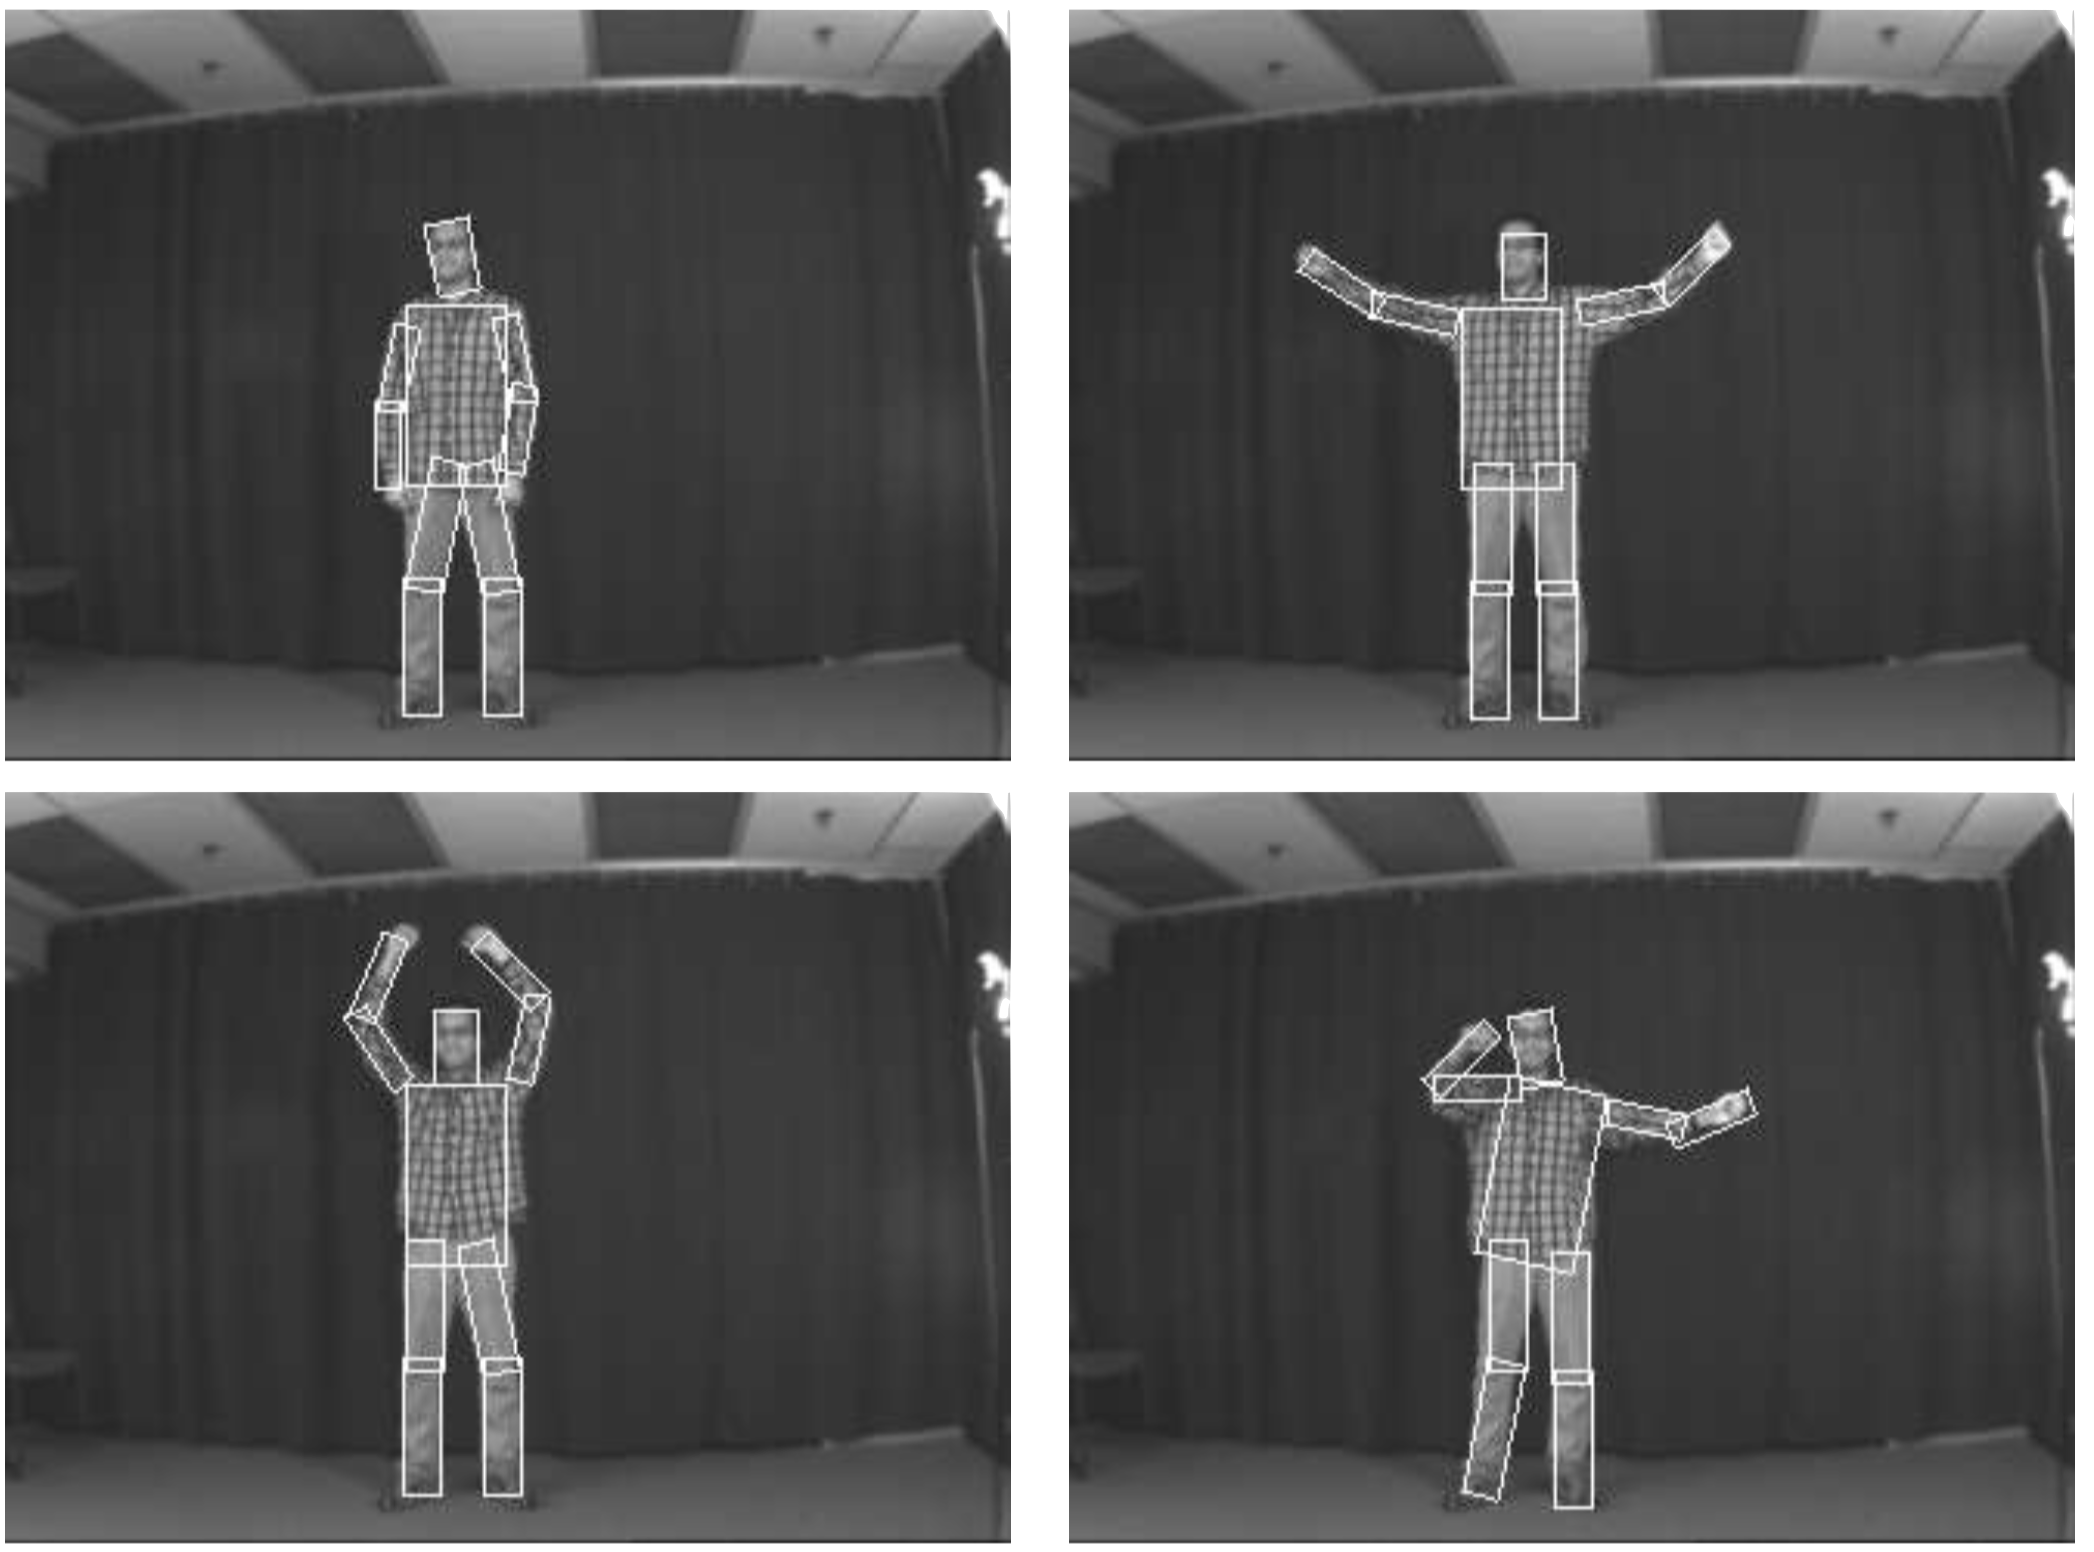
\includegraphics[width=.95\textwidth]{pictorial_structures.png}
\end{frame}


\begin{frame}[plain]
  \begin{tikzpicture}[remember picture,overlay]
    \node[at=(current page.center)] {
      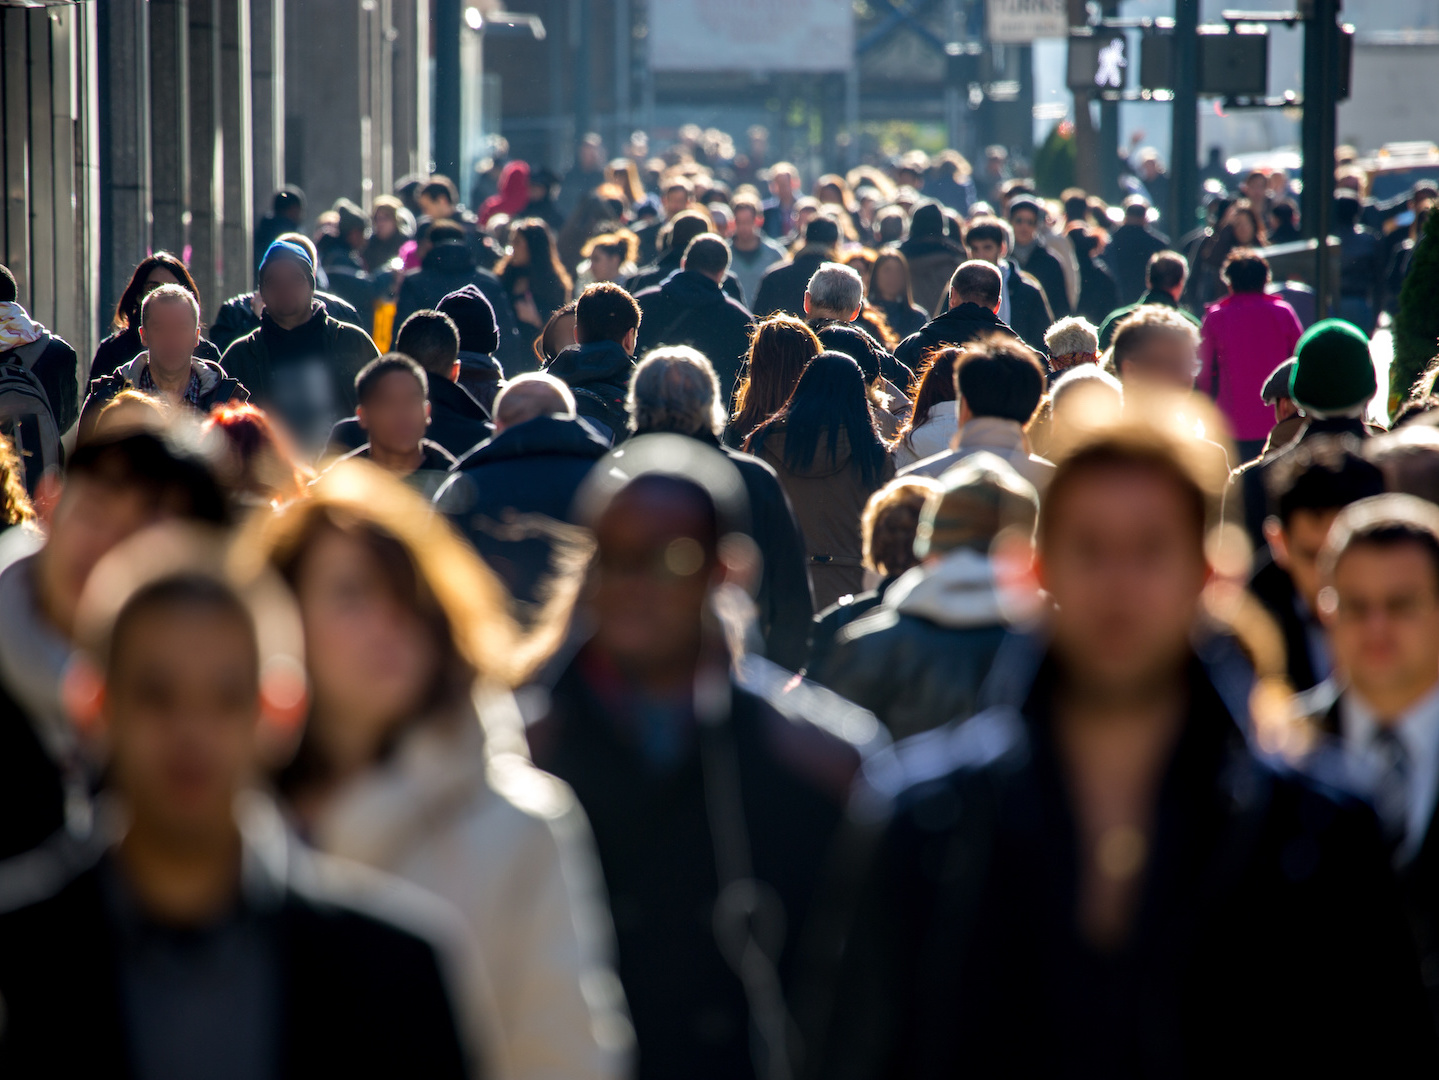
\includegraphics[width=\paperwidth]{crowd_street.jpg}
    };
  \end{tikzpicture}
\end{frame}

\section{Partial Occlusion Handling}
\label{sec:Partial Occlusion Handling}


\begin{frame}{Partial Occlusion Handling}
\small
\metroset{block=fill}

  \begin{alertblock}{\textbf{Why?}}
  Generally, especially in crowded scenes, occlusions occur frequently.
  Nevertheless, generic detectors, such as HOG, assume that pedestrians are fully
  visible and their performance degrades when pedestrians are partially occluded.
  \end{alertblock}
\pause

  \begin{exampleblock}{\textbf{How?}}
  The key to successful detection of partially occluded pedestrians is to use additional
  information about which body parts are occluded, for example \textit{correlations among
  the visibilities of different parts} having different sizes.
  \end{exampleblock}

\end{frame}


\begin{frame}{Partial Occlusion Handling}
  \metroset{block=fill}
  \begin{alertblock}{Probabilistic Framework}
    It models correlations among the visibilities of parts as hidden variables
  \end{alertblock}

\pause

  \begin{exampleblock}{Deep Model}
    The hierarchical structure of the deep model matches with the multilayers of
    the parts model well.
    Different from the other types of deep networks, whose hidden variables had
    no semantic meaning, this model considers each hidden variable as representing
    the visibility of a part.
  \end{exampleblock}

\end{frame}


\begin{frame}{A little bit of math}

Let $\mathbf{x}\in\mathbb{R}^d$ and $y\in\lbrace0,1\rbrace$ be respectively the \textit{feature vector} and the \textit{label} of a detection window.\\
\vspace{3mm}
\pause
Denote the detection scores of the $P$ parts by $\mathbf{s} = [s_1,...,s_P]^T = \gamma(\mathbf{x})$, where $\gamma(\mathbf{x})$ are part detectors.\\
\vspace{3mm}
\pause
Denote the visibilities of the $P$ parts by $\mathbf{h} = [h_1,...,h_P]^T \in\lbrace0,1\rbrace^P$, with $h_i = 1$ meaning \textbf{visible} and $h_i = 0$ meaning \textbf{invisible}.

\end{frame}


\begin{frame}{Hidden variable framework}
\begin{equation}
  p(y\vert\mathbf{x}) = \sum_\mathbf{h}p(y,\mathbf{h}\vert\mathbf{x}) = \sum_\mathbf{h}p(y\vert\mathbf{h},\mathbf{x})p(\mathbf{h}\vert\mathbf{x})
\end{equation}

%\pause
%  Often, for a fast approximate solution, this relation is simplified as follows:
%\begin{equation}
%  p(y\vert\mathbf{x}) \approx \exp \left( \sum_i s_i \right)
%\end{equation}

\pause
\metroset{block=fill}
\begin{block}{Objective}
  Build a deep model that learns the correlation of visibility
   relationship among parts
\end{block}

\end{frame}

\begin{frame}{Deep Model for Part Visibility Estimation}
\centering
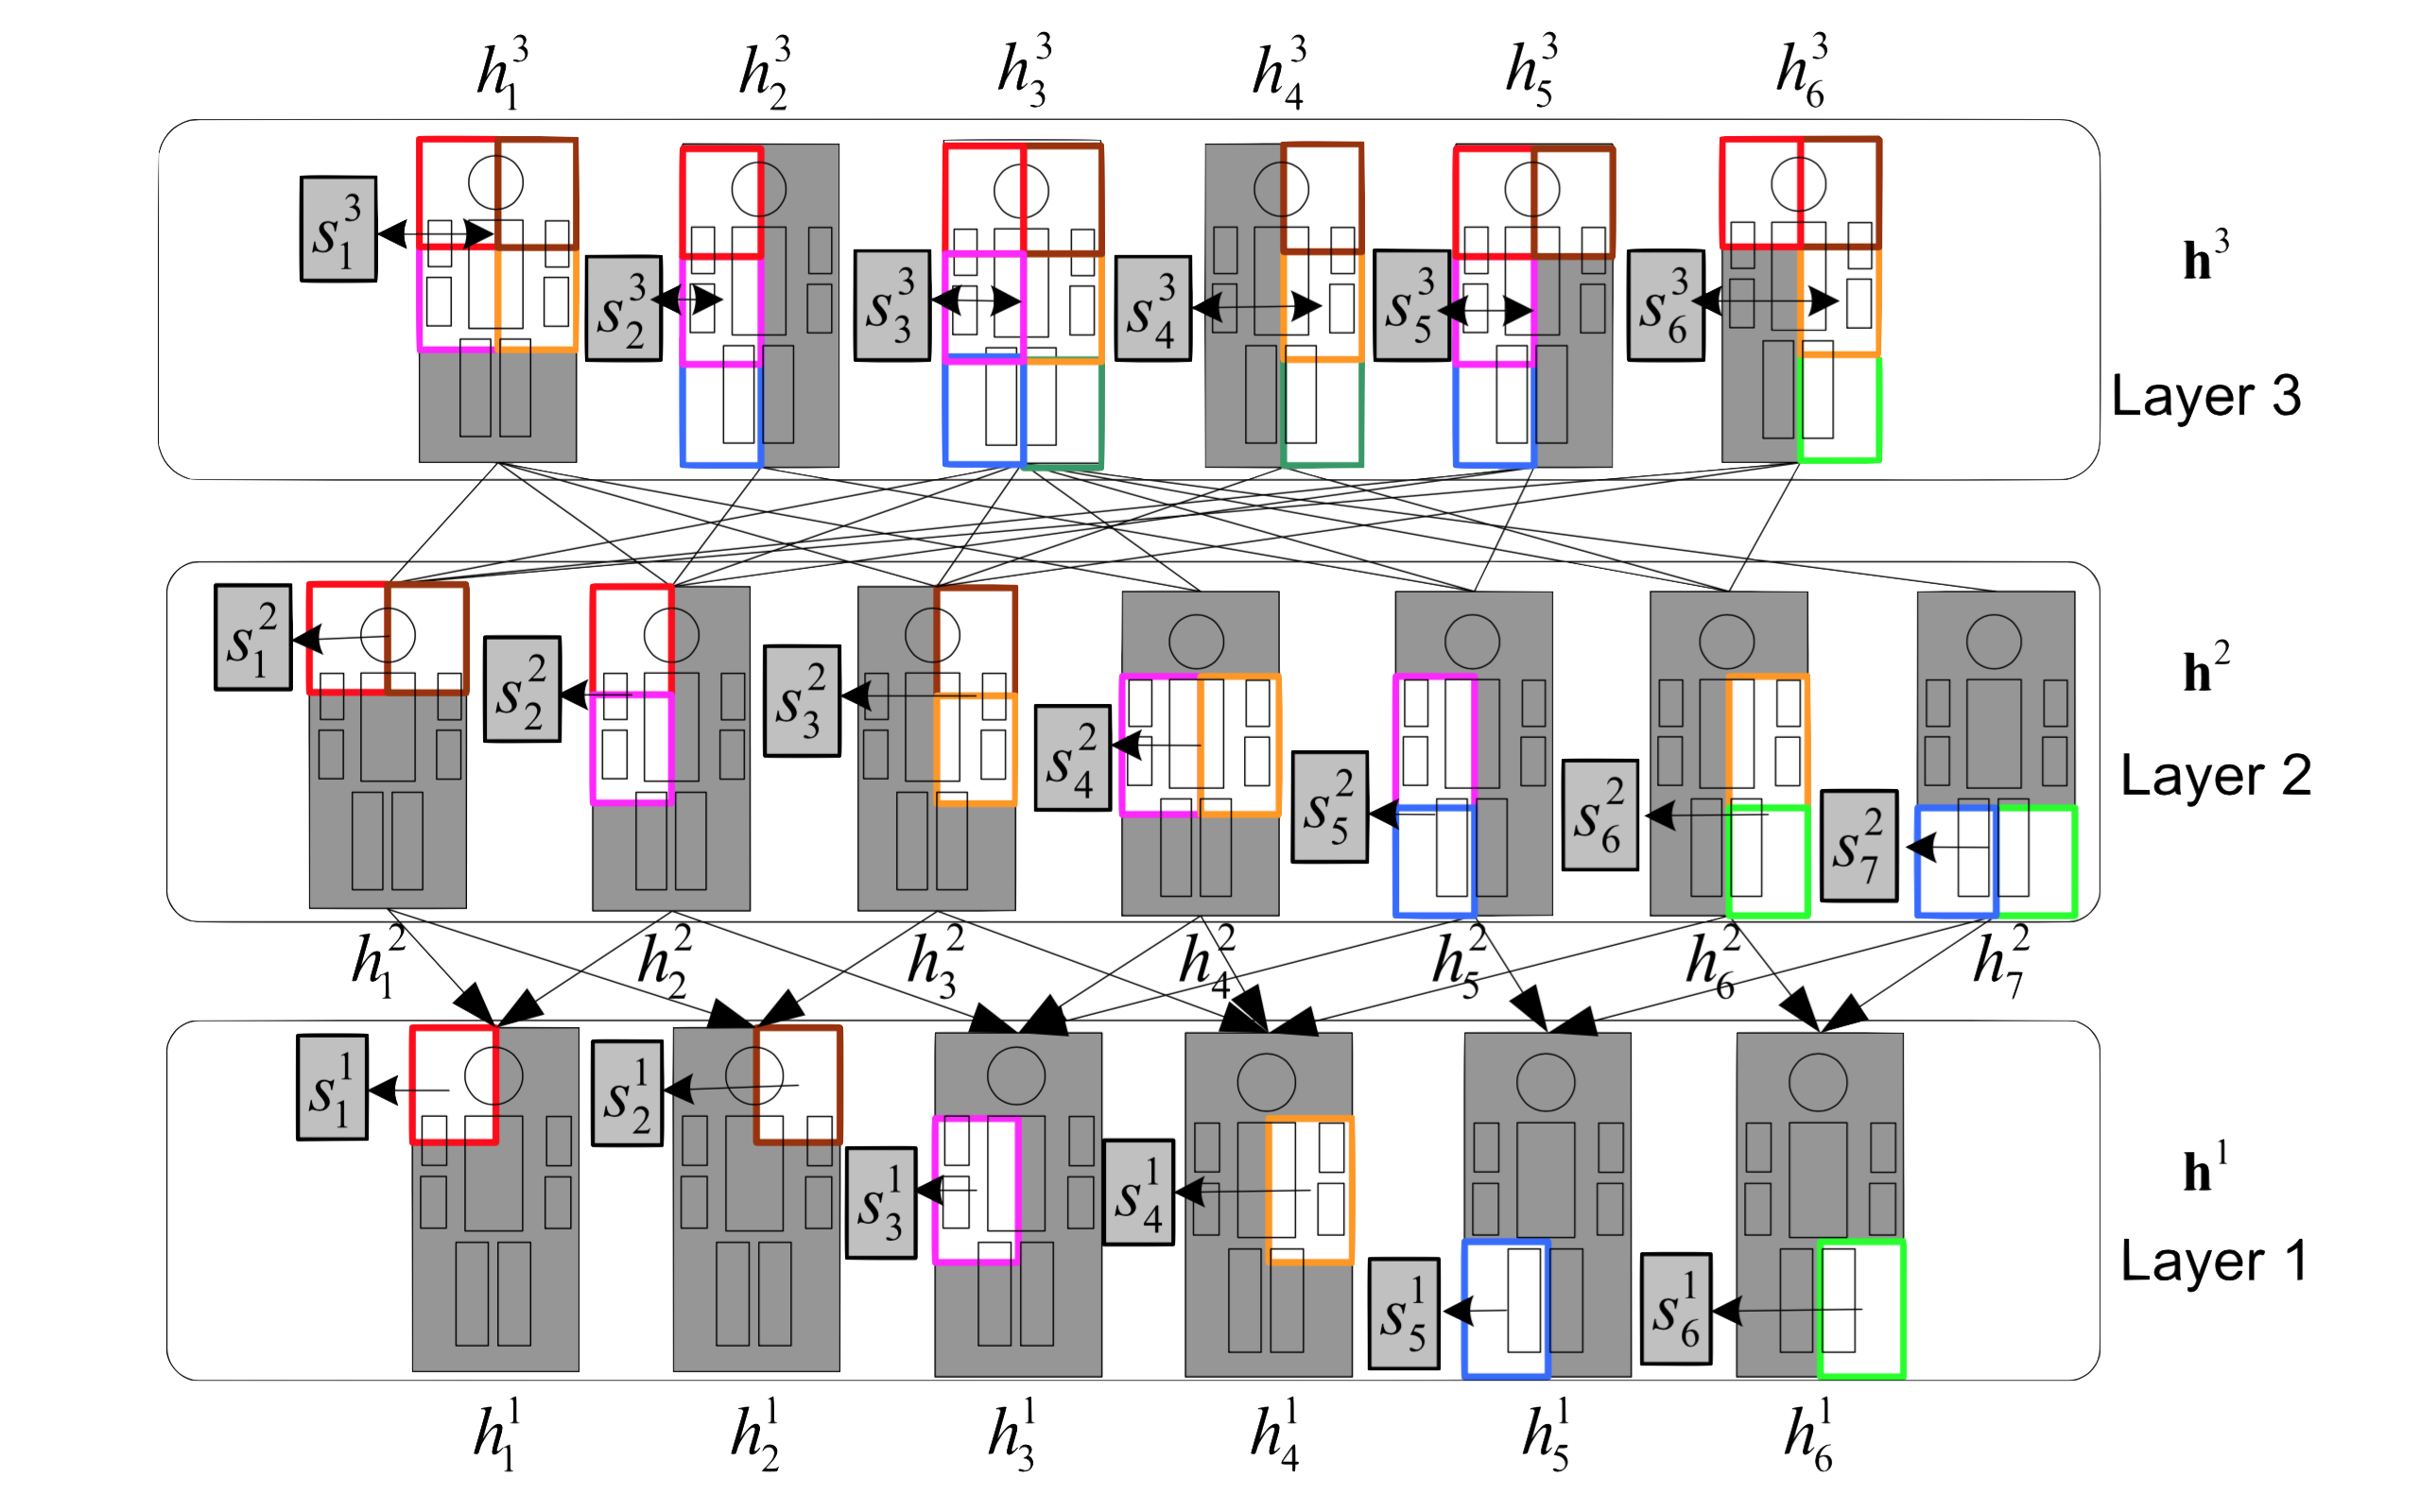
\includegraphics[width=0.85\textwidth]{mlp2.png}
\\
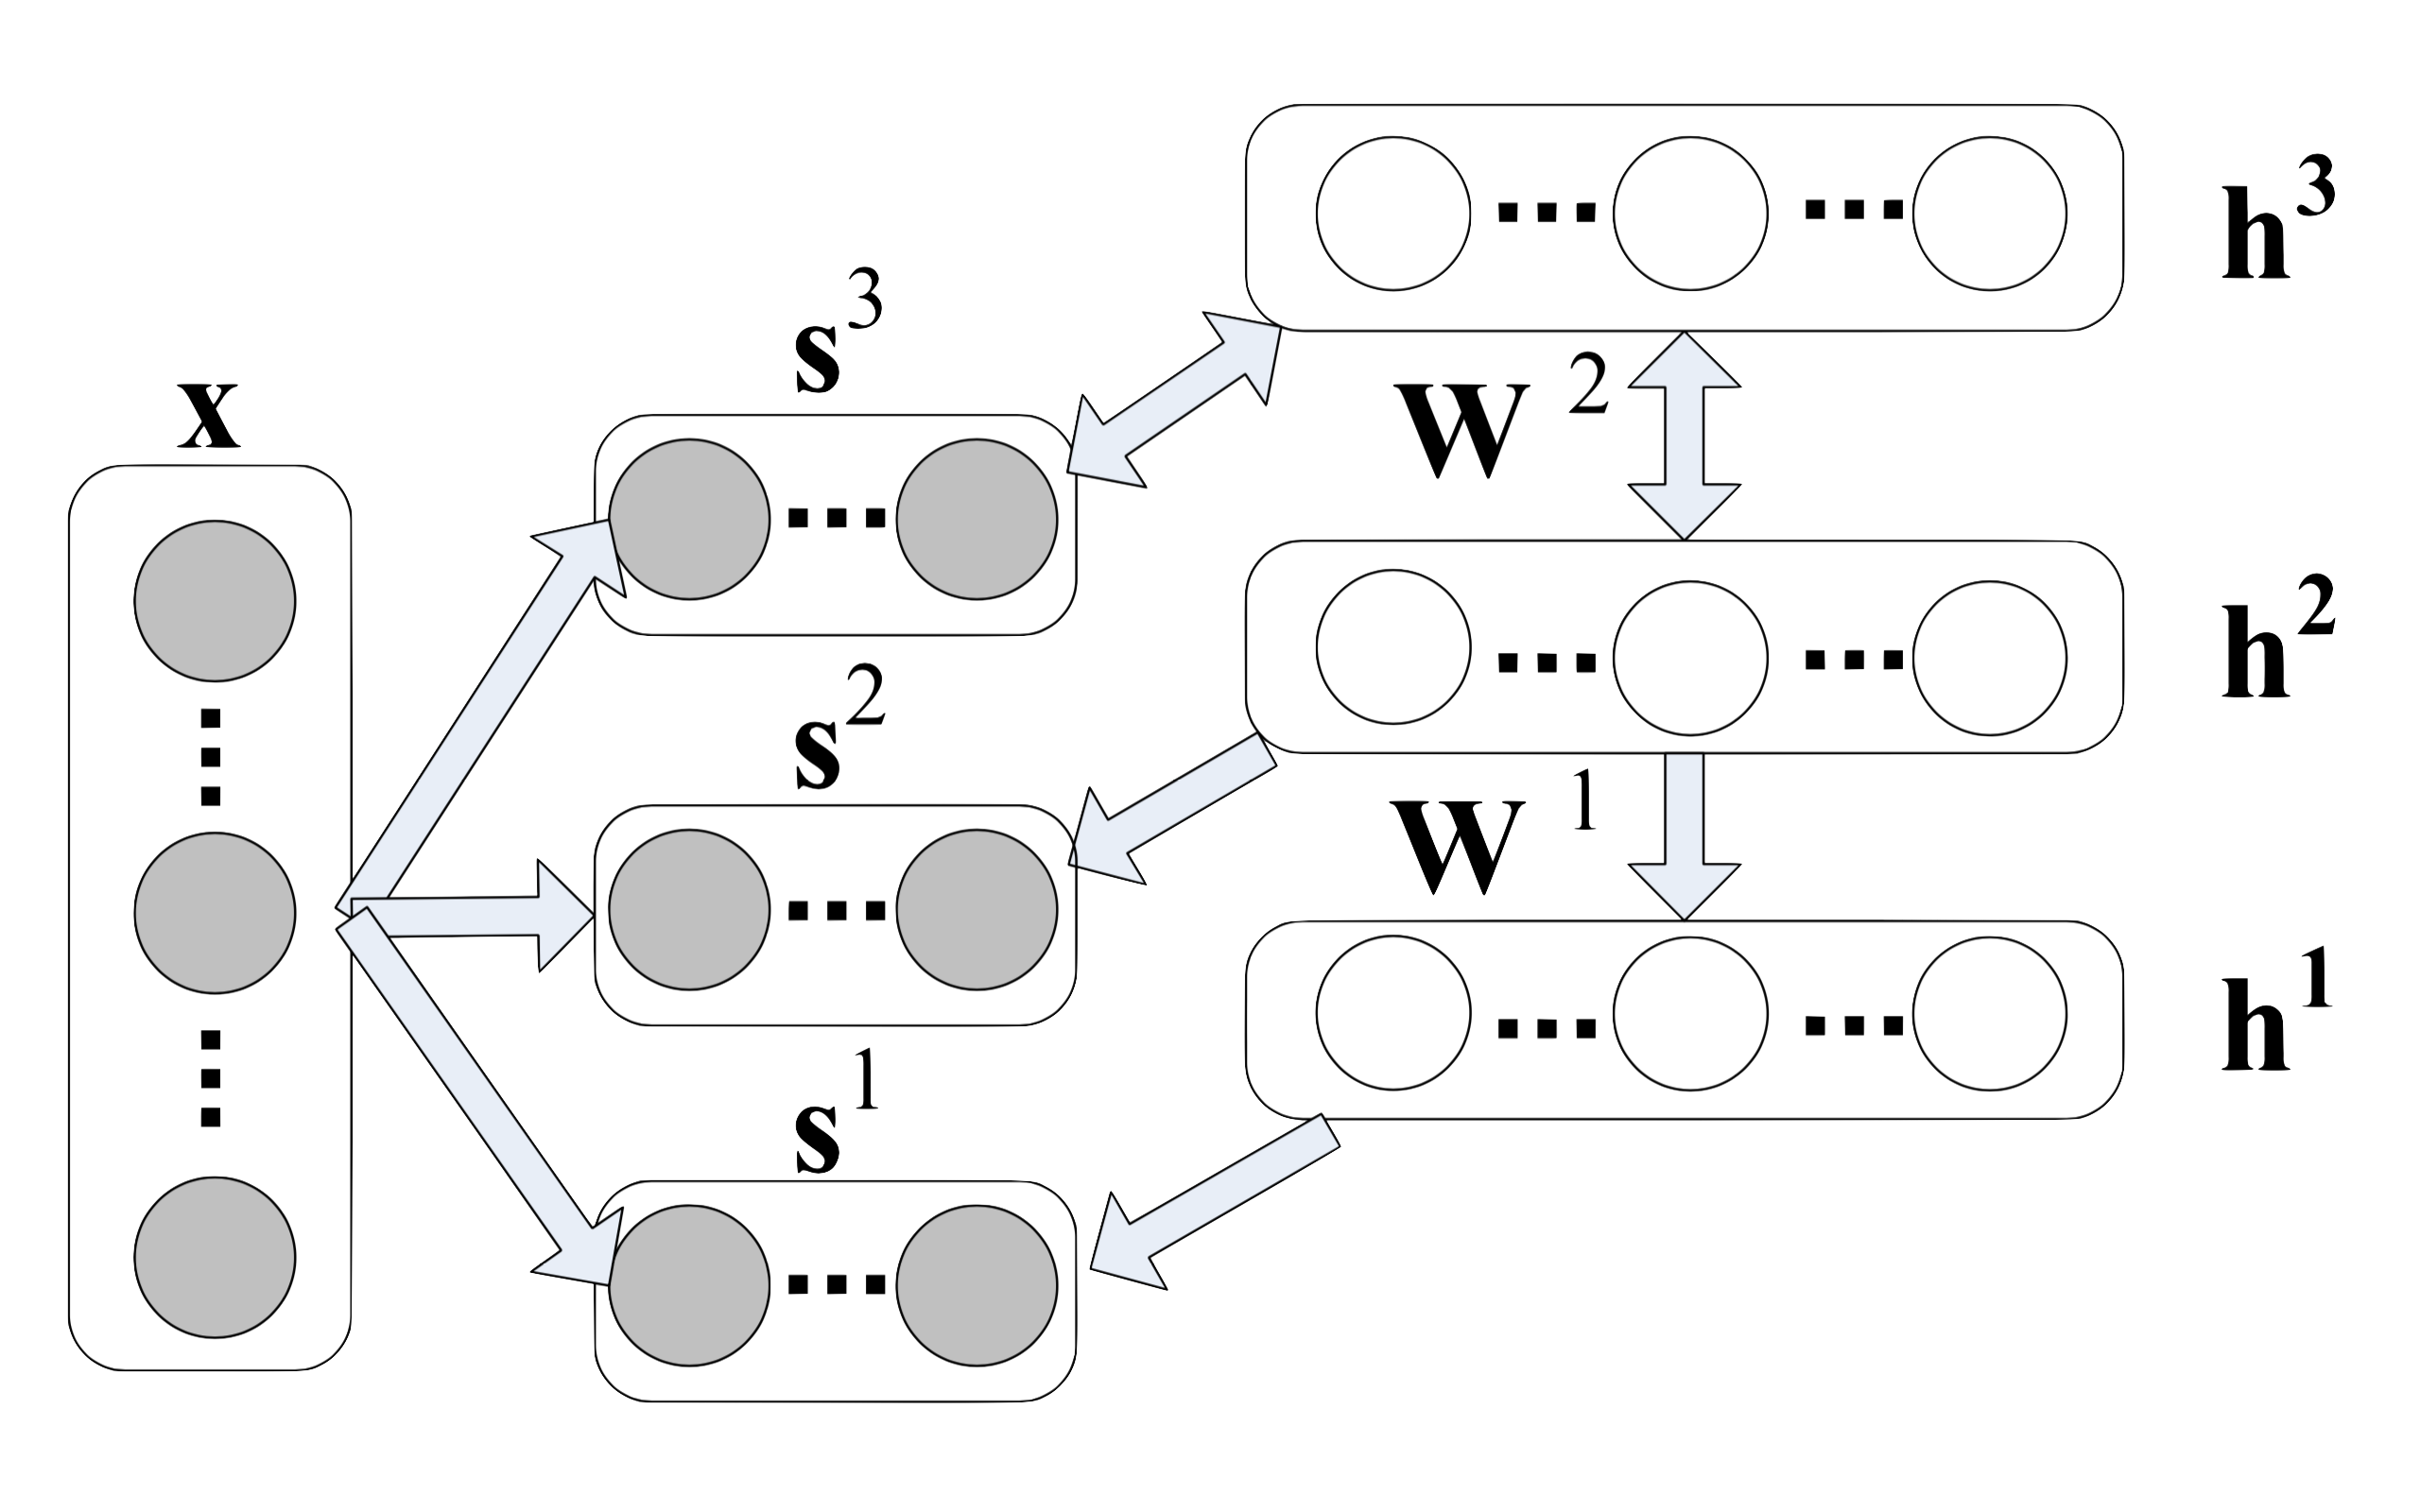
\includegraphics[width=0.3\textwidth]{mlp1.png}
\end{frame}

\begin{frame}{Result}
  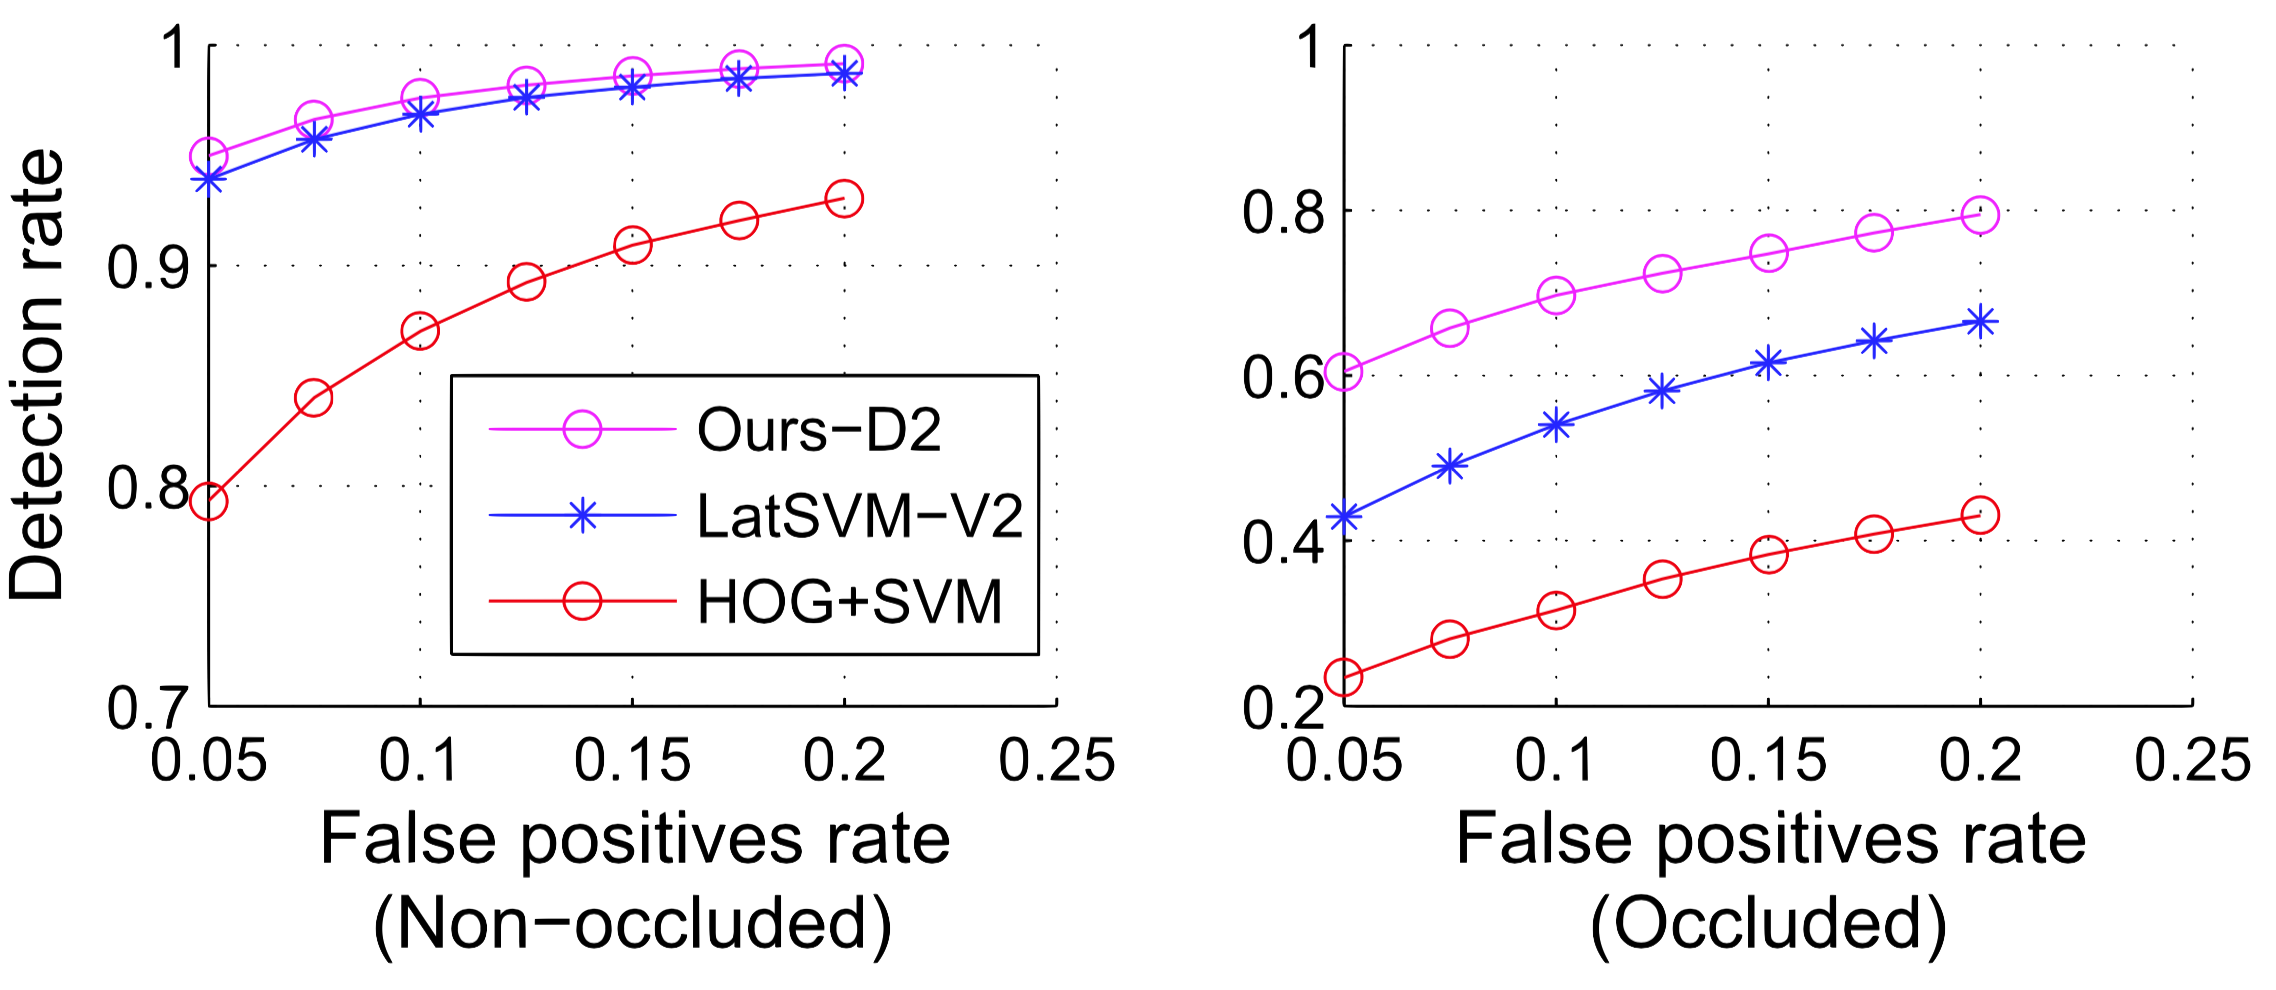
\includegraphics[width=\textwidth]{mlp_result.png}
\end{frame}



%\section{Titleformats}
%
%\begin{frame}{Metropolis titleformats}
%	\themename supports 4 different titleformats:
%	\begin{itemize}
%		\item Regular
%		\item \textsc{Smallcaps}
%		\item \textsc{allsmallcaps}
%		\item ALLCAPS
%	\end{itemize}
%	They can either be set at once for every title type or individually.
%\end{frame}
%
%{
%    \metroset{titleformat frame=smallcaps}
%\begin{frame}{Small caps}
%	This frame uses the \texttt{smallcaps} titleformat.
%
%	\begin{alertblock}{Potential Problems}
%		Be aware, that not every font supports small caps. If for example you typeset your presentation with pdfTeX and the Computer Modern Sans Serif font, every text in smallcaps will be typeset with the Computer Modern Serif font instead.
%	\end{alertblock}
%\end{frame}
%}
%
%{
%\metroset{titleformat frame=allsmallcaps}
%\begin{frame}{All small caps}
%	This frame uses the \texttt{allsmallcaps} titleformat.
%
%	\begin{alertblock}{Potential problems}
%		As this titleformat also uses smallcaps you face the same problems as with the \texttt{smallcaps} titleformat. Additionally this format can cause some other problems. Please refer to the documentation if you consider using it.
%
%		As a rule of thumb: Just use it for plaintext-only titles.
%	\end{alertblock}
%\end{frame}
%}
%
%{
%\metroset{titleformat frame=allcaps}
%\begin{frame}{All caps}
%	This frame uses the \texttt{allcaps} titleformat.
%
%	\begin{alertblock}{Potential Problems}
%		This titleformat is not as problematic as the \texttt{allsmallcaps} format, but basically suffers from the same deficiencies. So please have a look at the documentation if you want to use it.
%	\end{alertblock}
%\end{frame}
%}
%
%\section{Elements}
%
%\begin{frame}[fragile]{Typography}
%      \begin{verbatim}The theme provides sensible defaults to
%\emph{emphasize} text, \alert{accent} parts
%or show \textbf{bold} results.\end{verbatim}
%
%  \begin{center}becomes\end{center}
%
%  The theme provides sensible defaults to \emph{emphasize} text,
%  \alert{accent} parts or show \textbf{bold} results.
%\end{frame}
%
%\begin{frame}{Font feature test}
%  \begin{itemize}
%    \item Regular
%    \item \textit{Italic}
%    \item \textsc{SmallCaps}
%    \item \textbf{Bold}
%    \item \textbf{\textit{Bold Italic}}
%    \item \textbf{\textsc{Bold SmallCaps}}
%    \item \texttt{Monospace}
%    \item \texttt{\textit{Monospace Italic}}
%    \item \texttt{\textbf{Monospace Bold}}
%    \item \texttt{\textbf{\textit{Monospace Bold Italic}}}
%  \end{itemize}
%\end{frame}
%
%\begin{frame}{Lists}
%  \begin{columns}[T,onlytextwidth]
%    \column{0.33\textwidth}
%      Items
%      \begin{itemize}
%        \item Milk \item Eggs \item Potatos
%      \end{itemize}
%
%    \column{0.33\textwidth}
%      Enumerations
%      \begin{enumerate}
%        \item First, \item Second and \item Last.
%      \end{enumerate}
%
%    \column{0.33\textwidth}
%      Descriptions
%      \begin{description}
%        \item[PowerPoint] Meeh. \item[Beamer] Yeeeha.
%      \end{description}
%  \end{columns}
%\end{frame}
%\begin{frame}{Animation}
%  \begin{itemize}[<+- | alert@+>]
%    \item \alert<4>{This is\only<4>{ really} important}
%    \item Now this
%    \item And now this
%  \end{itemize}
%\end{frame}
%\begin{frame}{Figures}
%  \begin{figure}
%    \newcounter{density}
%    \setcounter{density}{20}
%    \begin{tikzpicture}
%      \def\couleur{alerted text.fg}
%      \path[coordinate] (0,0)  coordinate(A)
%                  ++( 90:5cm) coordinate(B)
%                  ++(0:5cm) coordinate(C)
%                  ++(-90:5cm) coordinate(D);
%      \draw[fill=\couleur!\thedensity] (A) -- (B) -- (C) --(D) -- cycle;
%      \foreach \x in {1,...,40}{%
%          \pgfmathsetcounter{density}{\thedensity+20}
%          \setcounter{density}{\thedensity}
%          \path[coordinate] coordinate(X) at (A){};
%          \path[coordinate] (A) -- (B) coordinate[pos=.10](A)
%                              -- (C) coordinate[pos=.10](B)
%                              -- (D) coordinate[pos=.10](C)
%                              -- (X) coordinate[pos=.10](D);
%          \draw[fill=\couleur!\thedensity] (A)--(B)--(C)-- (D) -- cycle;
%      }
%    \end{tikzpicture}
%    \caption{Rotated square from
%    \href{http://www.texample.net/tikz/examples/rotated-polygons/}{texample.net}.}
%  \end{figure}
%\end{frame}
%\begin{frame}{Tables}
%  \begin{table}
%    \caption{Largest cities in the world (source: Wikipedia)}
%    \begin{tabular}{lr}
%      \toprule
%      City & Population\\
%      \midrule
%      Mexico City & 20,116,842\\
%      Shanghai & 19,210,000\\
%      Peking & 15,796,450\\
%      Istanbul & 14,160,467\\
%      \bottomrule
%    \end{tabular}
%  \end{table}
%\end{frame}
%\begin{frame}{Blocks}
%  Three different block environments are pre-defined and may be styled with an
%  optional background color.
%
%  \begin{columns}[T,onlytextwidth]
%    \column{0.5\textwidth}
%      \begin{block}{Default}
%        Block content.
%      \end{block}
%
%      \begin{alertblock}{Alert}
%        Block content.
%      \end{alertblock}
%
%      \begin{exampleblock}{Example}
%        Block content.
%      \end{exampleblock}
%
%    \column{0.5\textwidth}
%
%      \metroset{block=fill}
%
%      \begin{block}{Default}
%        Block content.
%      \end{block}
%
%      \begin{alertblock}{Alert}
%        Block content.
%      \end{alertblock}
%
%      \begin{exampleblock}{Example}
%        Block content.
%      \end{exampleblock}
%
%  \end{columns}
%\end{frame}
%\begin{frame}{Math}
%  \begin{equation*}
%    e = \lim_{n\to \infty} \left(1 + \frac{1}{n}\right)^n
%  \end{equation*}
%\end{frame}
%\begin{frame}{Line plots}
%  \begin{figure}
%    \begin{tikzpicture}
%      \begin{axis}[
%        mlineplot,
%        width=0.9\textwidth,
%        height=6cm,
%      ]
%
%        \addplot {sin(deg(x))};
%        \addplot+[samples=100] {sin(deg(2*x))};
%
%      \end{axis}
%    \end{tikzpicture}
%  \end{figure}
%\end{frame}
%\begin{frame}{Bar charts}
%  \begin{figure}
%    \begin{tikzpicture}
%      \begin{axis}[
%        mbarplot,
%        xlabel={Foo},
%        ylabel={Bar},
%        width=0.9\textwidth,
%        height=6cm,
%      ]
%
%      \addplot plot coordinates {(1, 20) (2, 25) (3, 22.4) (4, 12.4)};
%      \addplot plot coordinates {(1, 18) (2, 24) (3, 23.5) (4, 13.2)};
%      \addplot plot coordinates {(1, 10) (2, 19) (3, 25) (4, 15.2)};
%
%      \legend{lorem, ipsum, dolor}
%
%      \end{axis}
%    \end{tikzpicture}
%  \end{figure}
%\end{frame}
%\begin{frame}{Quotes}
%  \begin{quote}
%    Veni, Vidi, Vici
%  \end{quote}
%\end{frame}
%
%{%
%\setbeamertemplate{frame footer}{My custom footer}
%\begin{frame}[fragile]{Frame footer}
%    \themename defines a custom beamer template to add a text to the footer. It can be set via
%    \begin{verbatim}\setbeamertemplate{frame footer}{My custom footer}\end{verbatim}
%\end{frame}
%}
%
%\begin{frame}{References}
%  Some references to showcase [allowframebreaks] \cite{knuth92,ConcreteMath,Simpson,Er01,greenwade93}
%\end{frame}
%
%\section{Conclusion}
%
%\begin{frame}{Summary}
%
%  Get the source of this theme and the demo presentation from
%
%  \begin{center}\url{github.com/matze/mtheme}\end{center}
%
%  The theme \emph{itself} is licensed under a
%  \href{http://creativecommons.org/licenses/by-sa/4.0/}{Creative Commons
%  Attribution-ShareAlike 4.0 International License}.
%
%  \begin{center}\ccbysa\end{center}
%
%\end{frame}
%
%\begin{frame}[standout]
%  Questions?
%\end{frame}
%
%\appendix
%
%\begin{frame}[fragile]{Backup slides}
%  Sometimes, it is useful to add slides at the end of your presentation to
%  refer to during audience questions.
%
%  The best way to do this is to include the \verb|appendixnumberbeamer|
%  package in your preamble and call \verb|\appendix| before your backup slides.
%
%  \themename will automatically turn off slide numbering and progress bars for
%  slides in the appendix.
%\end{frame}
%
%\begin{frame}[allowframebreaks]{References}
%
%  \bibliography{learning_to_drive}
%  \bibliographystyle{abbrv}
%
%\end{frame}
%
\end{document}
%
